%% LaTeX Paper Template, Flip Tanedo (flip.tanedo@ucr.edu)
%% GitHub: https://github.com/fliptanedo/paper-template-2022

\documentclass[12pt]{article}

%!TEX root = paper.tex
%% FLIP’S PREAMBLE; 
%% Use FlipAdditionalHeader for project-specific packages & macros

% \pdfoutput=1 % for JHEP

%%%%%%%%%%%%%%%%%%%%%%%%%%
%%%  COMMON PACKAGES  %%%%
%%%%%%%%%%%%%%%%%%%%%%%%%%

\usepackage{amsmath}
\usepackage{amssymb}
\usepackage{amsfonts}
\usepackage{graphicx}
\usepackage[utf8]{inputenc}     % inspire bibs
\usepackage{aas_macros}				  % ads bibs
\usepackage{bm}                 % \boldsymbol
\usepackage{amsthm}
\usepackage{microtype}

%%%%%%%%%%%%%%%%%%%%%%%%%%%
%%%  UNUSUAL PACKAGES  %%%%
%%%%%%%%%%%%%%%%%%%%%%%%%%%

%% MATH AND PHYSICS SYMBOLS
%% ------------------------
\usepackage{slashed}				% \slashed{k}
\usepackage{mathrsfs}				% Weinberg-esque letters
\usepackage{bbm}					  % \mathbbm{1} conflict: XeLaTeX 
\usepackage{cancel}					
\usepackage[normalem]{ulem} % for \sout
\usepackage{youngtab}	    	% Young Tableaux

%% CONTENT FORMAT AND DESIGN
%% -------------------------
\usepackage[dvipsnames]{xcolor}
\usepackage[hang,flushmargin]{footmisc} % no footnote indent

\usepackage{fancyhdr}		% preprint number
\usepackage{lipsum}			% block of text 
\usepackage{framed}			% boxed remarks / Next time: use mdframed
                        % https://github.com/marcodaniel/mdframed/blob/master/mdframed.pdf
\usepackage{subcaption}	% subfigures
\usepackage{cite}			  % group cites
\usepackage{xspace}			% macro spacing


%% TABLES IN LaTeX
%% ---------------
\usepackage{booktabs}		% professional tables
\usepackage{nicefrac}		% fractions in tables,
\usepackage{multirow}		% multirow elements in a table
\usepackage{arydshln}		% dashed lines in arrays

%% ARRAY STRETCH: vertical spacing between rows
% \renewcommand{\arraystretch}{1.5} %% put this in main text

%% Other Packages and Notes
%% ------------------------
\usepackage[font=small]{caption} 	% caption font is small
\usepackage{float}         			  % for strict placement e.g. [H]


%%%%%%%%%%%%%%%%%%%%%%%%%%%%%%
%%%  DOCUMENT PROPERTIES  %%%%
%%%%%%%%%%%%%%%%%%%%%%%%%%%%%%

\usepackage[margin=2.5cm]{geometry} % margins
\graphicspath{{figures/}}			      % figure folder
\numberwithin{equation}{section}    % set equation numbering
% \usepackage{marginnote}             % for \marginnote{comment}
% \usepackage{mparhack}               % fix for \marginnote
% \usepackage{marginfix}              % fix for \marginnote
% \usepackage{adjustbox}              % to rescale elements



%% References in two columns, smaller
%% http://tex.stackexchange.com/questions/20758/
\usepackage{multicol}
\usepackage{etoolbox}
\usepackage{relsize}
\patchcmd{\thebibliography}
  {\list}
  {\begin{multicols}{2}\smaller\list}
  {}
  {}
\appto{\endthebibliography}{\end{multicols}}


% Change list spacing (instead of package paralist)
% from: http://en.wikibooks.org/wiki/LaTeX/List_Structures#Line_spacing
% alternative: enumitem package
\let\oldenumerate\enumerate
\renewcommand{\enumerate}{
  \oldenumerate
  \setlength{\itemsep}{4pt}
  \setlength{\parskip}{0pt}
  \setlength{\parsep}{0pt}
}

\let\olditemize\itemize
\renewcommand{\itemize}{
  \olditemize
  \setlength{\itemsep}{4pt}
  \setlength{\parskip}{0pt}
  \setlength{\parsep}{0pt}
}

%% FOR DRAFT EDITING AND DISCUSSION
\usepackage{lineno}
% \linenumbers          %% put this in main text


%%%%%%%%%%%%%%%%%%%%%%%%%%%
%%%  (RE)NEW COMMANDS  %%%%
%%%%%%%%%%%%%%%%%%%%%%%%%%%

%% FOR `NOT SHOUTING' CAPS (e.g. acronyms)
%% ---------------------------------------
\usepackage{scalefnt} 
\newcommand\acro[1]{{\footnotesize #1}}           % acronyms in footnote size


%% COMMON PHYSICS MACROS
%% ---------------------
\renewcommand{\tilde}{\widetilde}                 % tilde over characters
\renewcommand{\text}{\textnormal}	                % text in equations 
\renewcommand{\vec}[1]{\mathbf{#1}}               % vectors are boldface

%% Differential and differential/2pi
% \newcommand{\dbar}{d\mkern-6mu\mathchar'26}     % for d/2pi
\newcommand{\dbar}{d\mkern-6mu\mathchar'26\hspace{-.1em}}    
%% Best practice: Roman differential
\newcommand{\D}[1]{\ensuremath{\operatorname{d}\!{#1}}}
\newcommand{\Dbar}[1]{\operatorname{d}\mkern-10mu\mathchar'26\mkern-2mu{#1}}    % fixed spacing
\newcommand{\ket}[1]{\left|#1\right\rangle}       % <#1|
\newcommand{\bra}[1]{\left\langle#1\right|}       % |#1>
\newcommand*{\trans}{\mkern-1.5mu\mathsf{T}}      % transpose

%% COMMANDS FOR TEMPORARY COMMENTS
%% -------------------------------
\newcommand{\comment}[2]{\textcolor{red}{[\textbf{#1} #2]}}
\newcommand{\flip}[1]{{
	\color{green!50!black}
  \footnotesize
  [\textbf{\textsf{Flip}}: \textsf{#1}]
	}}


%% COMMANDS FOR TOP-MATTER
%% -----------------------
\newcommand{\email}[1]{\href{mailto:#1}{#1}}
\newenvironment{institutions}[1][2em]{\begin{list}{}{\setlength\leftmargin{#1}\setlength\rightmargin{#1}}\item[]}{\end{list}}


%% COMMANDS FOR LATEXDIFF
%% ----------------------
%% see http://bit.ly/1M74uwc
\providecommand{\DIFadd}[1]{{\protect\color{blue}#1}} %DIF PREAMBLE
\providecommand{\DIFdel}[1]{{\protect\color{red}\protect\scriptsize{#1}}}

%% REMARK: use latexdiff option --allow-spaces
%% for \frac, ref: http://bit.ly/1iFlujR
%% Errors with environments? https://tex.stackexchange.com/q/73224

%% USAGE: latexdiff draft.tex revision.tex > diff.tex

%%%%%%%%%%%%%%%%%%%%%
%%%  TITLE DATA  %%%%
%%%%%%%%%%%%%%%%%%%%%

%% PREPRINT NUMBER USING fancyhdr
%% Don't forget to set \thispagestyle{firststyle}
%% ----------------------------------------------
\renewcommand{\headrulewidth}{0pt} 	% no separator
\setlength{\headheight}{15pt} 		% min to avoid fancyhdr warning
\fancypagestyle{firststyle}{
	\rhead{\footnotesize%
	\texttt{\FlipTR}%
	}}

%% TOC overwrites fancyhdr, here's a fix
%% http://tex.stackexchange.com/questions/167828/
\usepackage{etoc}
\renewcommand{\etocaftertitlehook}{\pagestyle{plain}}
\renewcommand{\etocaftertochook}{\thispagestyle{firststyle}}			%% \usepackages
%!TEX root = paper.tex
%% Update the above with the appropriate root

%% Place additional project-specific macros, package calls here
%% These are called before FlipPreambleEnd.tex so that,
%% for example, they are called before hyperref


%% FIGURE SNIPPIT
% \begin{figure}[tb]
%     \centering
%     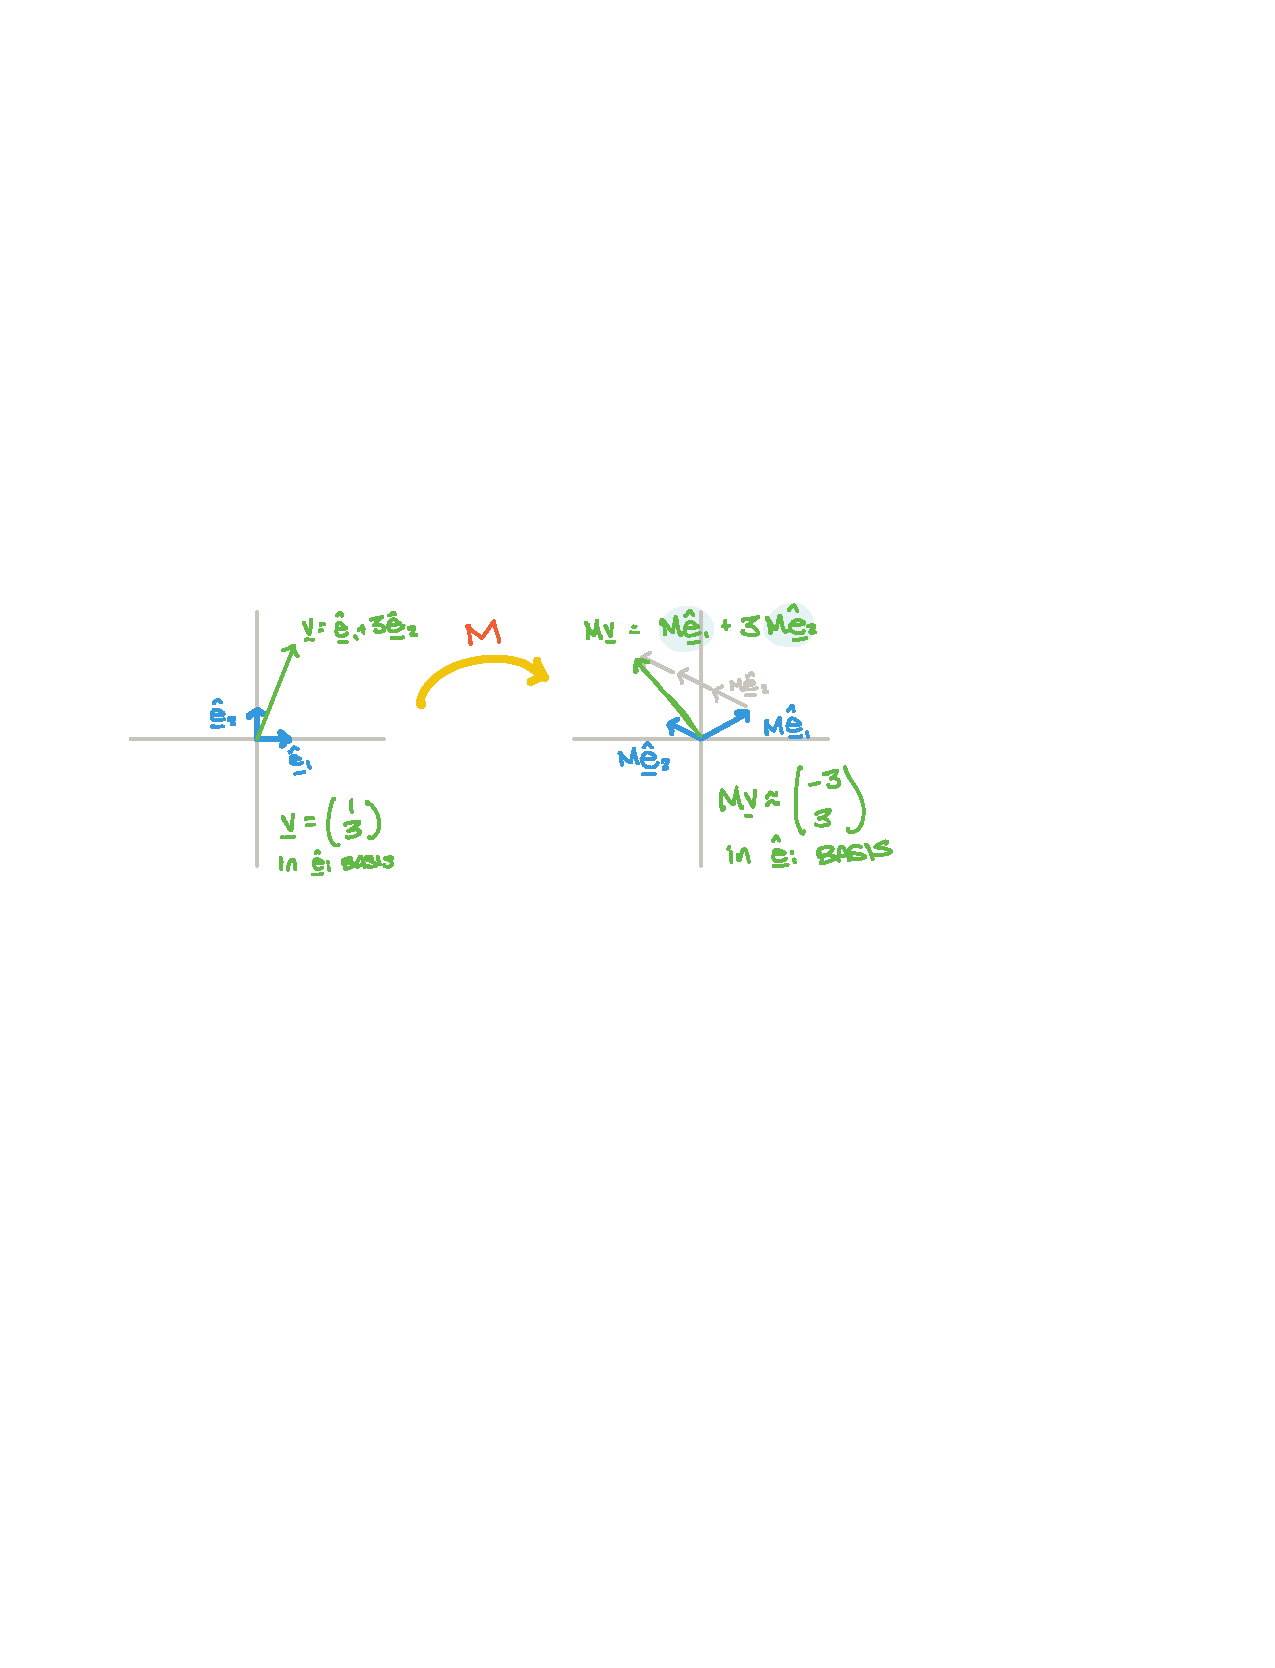
\includegraphics[width=.8\textwidth]{figures/maps_M.pdf}
%     \caption{.}
%     \label{fig:}
% \end{figure}

%% THEOREM ENVIRONMENTS


%% Because mdframed causes a bunch of warnings
%% https://tex.stackexchange.com/questions/64331/disable-warning-from-mdframed 
\usepackage{silence}
\WarningFilter{mdframed}{You got a bad break}
\WarningFilter{mdframed}{correct box splittet fails}



\newmdtheoremenv[
    skipabove=2em,
    skipbelow=2em,
    linewidth=5pt,
    linecolor=red!50!black,
    topline=false,
    rightline=false,
    bottomline=false
    ]{exercise}{Exercise}[section]


\newmdtheoremenv[
    skipabove=2em,
    skipbelow=2em,
    linewidth=5pt,
    linecolor=gray,
    topline=false,
    rightline=false,
    bottomline=false
    ]{example}{Example}[section]

\newmdtheoremenv[
    skipabove=2em,
    skipbelow=2em,
    linewidth=5pt,
    linecolor=blue,
    topline=false,
    rightline=false,
    bottomline=false
    ]{bigidea}{Key Idea}[section]
\newcommand{\bigidearef}{Key~Idea\xspace}
\newcommand{\bigidearefs}{Key~Ideas\xspace}

%% AMS Theorem version
% \newtheorem{exercise}{Exercise}[section]
% \newtheorem{example}{Example}[section]

%% Example: replace YourName with your name
\newcommand{\YourName}[1]{{	
	\color{blue!50!black}\footnotesize
	[\textbf{\textsf{YourName}}: \textsf{#1}]}}


\renewcommand{\tilde}{\widetilde}   % tilde over characters
\renewcommand{\vec}[1]{\mathbf{#1}} % vectors are boldface
\newcommand{\bas}[1]{\hat{\mathbf{#1}}} 	% basis vectors have hat
\newcommand{\row}[1]{\tilde{\mathbf{#1}}} 	% row vectors have tilde

% For matrices
\newcommand{\aij}[2]{^{#1}_{\phantom{#1}#2}}
\newcommand{\mat}[3]{#1\aij{#2}{#3}}
\newcommand{\pp}{\phantom{+}}
\newcommand{\inv}{^{-1}}


\usepackage{pifont}
	\newcommand{\cmark}{\ding{51}}%
	\newcommand{\xmark}{\ding{55}}%


%% COMMANDS FOR TEMPORARY COMMENTS
%% -------------------------------
\newcommand{\comment}[2]{\textcolor{red}{[\textbf{#1} #2]}}
\newcommand{\flip}[1]{{
	\color{green!50!black}
  \footnotesize
  [\textbf{\textsf{Flip}}: \textsf{#1}]
	}}

\newcommand{\correction}[2]{{
	\color{green!50!black}
  \footnotesize
  [\textbf{\textsf{Correction,~#1}}: \textsf{#2}]
	}}
 	%% Use this define additional macros
% %!TEX root = paper.tex
%% Update the above with the appropriate root


%% LISTINGS PACKAGE
%% https://www.overleaf.com/learn/latex/Code_listing
%% https://tex.stackexchange.com/a/350242
\usepackage{xcolor}
\usepackage[most]{tcolorbox}
\usepackage{listings}

\definecolor{white}{rgb}{1,1,1}
\definecolor{mygreen}{rgb}{0,0.4,0}
\definecolor{light_gray}{rgb}{0.97,0.97,0.97}
\definecolor{mykey}{rgb}{0.117,0.403,0.713}

\tcbuselibrary{listings}
\newlength\inwd
\setlength\inwd{1.3cm}

\newcounter{ipythcntr}
\renewcommand{\theipythcntr}{\texttt{[\arabic{ipythcntr}]}}

\newtcblisting{pyin}[1][]{%
  sharp corners,
  enlarge left by=\inwd,
  width=\linewidth-\inwd,
  enhanced,
  boxrule=0pt,
  colback=light_gray,
  listing only,
  top=0pt,
  bottom=0pt,
  overlay={
    \node[
      anchor=north east,
      text width=\inwd,
      font=\footnotesize\ttfamily\color{mykey},
      inner ysep=2mm,
      inner xsep=0pt,
      outer sep=0pt
      ] 
      at (frame.north west)
      {\refstepcounter{ipythcntr}\label{#1}In \theipythcntr:};
  }
  listing engine=listing,
  listing options={
    aboveskip=1pt,
    belowskip=1pt,
    basicstyle=\footnotesize\ttfamily,
    language=Python,
    keywordstyle=\color{mykey},
    showstringspaces=false,
    stringstyle=\color{mygreen}
  },
}
\newtcblisting{pyprint}{
  sharp corners,
  enlarge left by=\inwd,
  width=\linewidth-\inwd,
  enhanced,
  boxrule=0pt,
  colback=white,
  listing only,
  top=0pt,
  bottom=0pt,
  overlay={
    \node[
      anchor=north east,
      text width=\inwd,
      font=\footnotesize\ttfamily\color{mykey},
      inner ysep=2mm,
      inner xsep=0pt,
      outer sep=0pt
      ] 
      at (frame.north west)
      {};
  }
  listing engine=listing,
  listing options={
      aboveskip=1pt,
      belowskip=1pt,
      basicstyle=\footnotesize\ttfamily,
      language=Python,
      keywordstyle=\color{mykey},
      showstringspaces=false,
      stringstyle=\color{mygreen}
    },
}
\newtcblisting{pyout}[1][\theipythcntr]{
  sharp corners,
  enlarge left by=\inwd,
  width=\linewidth-\inwd,
  enhanced,
  boxrule=0pt,
  colback=white,
  listing only,
  top=0pt,
  bottom=0pt,
  overlay={
    \node[
      anchor=north east,
      text width=\inwd,
      font=\footnotesize\ttfamily\color{mykey},
      inner ysep=2mm,
      inner xsep=0pt,
      outer sep=0pt
      ] 
      at (frame.north west)
      {\setcounter{ipythcntr}{\value{ipythcntr}}Out#1:};
  }
  listing engine=listing,
  listing options={
      aboveskip=1pt,
      belowskip=1pt,
      basicstyle=\footnotesize\ttfamily,
      language=Python,
      keywordstyle=\color{mykey},
      showstringspaces=false,
      stringstyle=\color{mygreen}
    },
}


% amsthm details:


\newtheorem{exercise}{Exercise}[section]
\newtheorem{example}{Example}[section]

%!TEX root = paper.tex
%% These are packages that need to be called at the end of the preamble 
%% or else they may lead to potential package conflicts.

%%%%%%%%%%%%%%%%%%%
%%%  HYPERREF  %%%%
%%%%%%%%%%%%%%%%%%%

%% This package has to be at the end; can lead to conflicts
\usepackage[
	colorlinks=true,
	citecolor=green!50!black,
	linkcolor=NavyBlue!75!black,
	urlcolor=green!50!black,
	hypertexnames=false]{hyperref}

%%%%%%%%%%%%%%%%%%%%%%%%%%%%%%%%%%%%%%%%
%%%  Must be called after HYPERREF  %%%%
%%%%%%%%%%%%%%%%%%%%%%%%%%%%%%%%%%%%%%%%


\usepackage{orcidlink}			% orcid ID icon; after hyperref
\usepackage{cleveref}
\crefformat{equation}{(#2#1#3)}	% strip eq.~ 
\crefrangeformat{equation}{(#3#1#4\,--\,#5#2#6)} % strip eqs.~			%% packages that have to be at the end
\begin{document}

\newcommand{\FlipTR}{UCR-TR-2023-FLIP-00X} % (pdfsync may fail on 1st page)
	\thispagestyle{firststyle} 	% TR#; otherwise use \thispagestyle{empty}


%%%%%%%%%%%%%%%%%%%%%%%%
%%%  FRONTMATTER    %%%%
%%%%%%%%%%%%%%%%%%%%%%%%

\begin{center}
    {\huge \textbf{Linear Algebra for Physicists} \par}
    \vskip .5cm
    %!TEX root = paper.tex
%% Update the above with the appropriate root

%% This is the author list
%% We separate it to keep the main file clean; this is
%% not the part of the document that gets updated often.

\newcommand{\authorA}{Flip Tanedo}
\newcommand{\emailA}{flip.tanedo@ucr.edu}
\newcommand{\orcidA}{0000-0003-4642-2199}
\newcommand{\institutionA}{
		Department of Physics \& Astronomy, 
	    University of  California, Riverside, 
	    \acro{CA} 92521}

\newcommand{\authorB}{Your Name}
\newcommand{\emailB}{your.name@ucr.edu}
\newcommand{\orcidB}{0000-0003-4642-2200}
\newcommand{\institutionB}{
		Department of Physics \& Astronomy, 
	    University of  California, Elsewhere, 
	    \acro{CA} 99999}

\newcommand{\authorC}{Tu Nombre}
\newcommand{\emailC}{tu.nombre@ucr.edu}
\newcommand{\orcidC}{0000-0003-4642-2201}
\newcommand{\institutionC}{
		Department of Physics \& Astronomy, 
	    University of  California, Elsewhere, 
	    \acro{CA} 99999}

	\textbf{\authorA}%$^{a}$,
	% \textbf{\authorB}$^{b}$,
	% and
	% \textbf{\authorC}$^{c}$, 
	\\ 
	\texttt{\footnotesize \email{\emailA}}~\orcidlink{\orcidA}%,
	% \texttt{\footnotesize \email{\emailB}}~\orcidlink{\orcidB},
	% \texttt{\footnotesize \email{\emailC}}~\orcidlink{\orcidC}

	\vspace{-.8em}
    \begin{institutions}[1.7cm]
    \footnotesize
    { 
    	% $^{a}$
    	\textit{\institutionA} 
    	% \\ $^{b}$ \textit{\institutionB} 
    	% \\ $^{c}$ \textit{\institutionC} 
	}    
    \end{institutions}


\end{center}

\begin{abstract}
\noindent 
Lecture notes for Physics 17, a course on linear algebra in preparation for upper-division undergraduate physics coursework at \acro{UC R}iverside.
\end{abstract}

\small
\setcounter{tocdepth}{2}
\tableofcontents
\normalsize
%\clearpage


%%%%%%%%%%%%%%%%%%%%%
%%%  THE CONTENT  %%%
%%%%%%%%%%%%%%%%%%%%%

\section{Logistics}

At any time in this course, you should feel comfortable asking either of the following questions:
\begin{enumerate}
    \item Is it obvious that...?
    \item Why is this significant?
\end{enumerate}
The first question is the way to ask for on-the-spot clarification---I will either appreciate that I did not properly explain a subtle point, \emph{or} I will explain the intuition\footnote{Your sense of mathematical and physical intuition is incredibly valuable. This is one of the key traits that makes a physics training unique.} for why something should be obvious. The second question is a way to remind me that I may have \emph{lost sight of the forest for the trees}: I want this course to \emph{mathematically connect big ideas in physics}. Asking this question is a reminder that making those connections justifies the hard mathematical work we will put into the course.


Finally, I want to comment on the word \emph{obvious}. I write this often. It is somewhat dangerous because it can come off as being arrogant: \emph{this is so obvious to me, if you do not understand you must be deficient}. This is never the reason why I use that word. Instead, the word \emph{obvious} serves a very practical purpose. The goal of this class is not just to be able to ``do stuff'' (e.g.~diagonalize a symmetric matrix), but to also build that intuition that comes from a deeper understanding how the mathematics works. In this sense, every time I write the word \emph{obvious} it is a flag: I am saying something that---with the proper perspective---should be self-evident. If it is not self-evident, then you should stop to interrogate why it is not self-evident. Most likely there is something where a change in perspective may (1) make it obvious, and (2) in so doing deepen your understanding of the subject. So when you see the word `obvious,' I want you to do a quick check to confirm whether or not the statement is indeed obvious. If it is not, then welcome the opportunity to learn.\footnote{There is, of course, the possibility that what I have written is \emph{not} obvious. For example, if I have made a typo... in which case, please let me know.}

\section{Motivation}

Here are three incredibly significant equations in physics:
\begin{align}
    \vec{F} &= m\vec{a}
    &
    R_{\mu\nu} - \frac{1}{2}Rg_{\mu\nu} 
    &= \frac{8\pi G_\text{N}}{c^4} T_{\mu\nu}
    &
    \hat H |\Psi\rangle 
    &= E |\Psi\rangle \ .
    \label{eq:three:equations}
\end{align}
These are Newton's force law, Einstein's field equations, and the Schr\"odinger equation. They govern classical physics, general relativity, and quantum theory. 


Each equation looks rather unique: they seem to each be speaking their own mathematical language. Newton's law is written with boldfaced vectorial quantities $\vec{F} = (F_x, F_y, F_z)^T$ that should look very familiar to any physics undergraduate. Einstein's equation has these funny $\mu$ and $\nu$ indices on every term---have you seen these before? Do they look intimidating? If you ever want to make your equations look ``technical'' and ``physicsy,'' you should dress them up with indices. The Schr\"odinger equation has no indices, but instead has these funny angle-brackety things... and that $\hat H$ looks suspicious. Where did $H$ get a hat, and what is the content of this equation other than $\hat H = E$?

\emph{Each of these equations turns out to be a ``vectorial'' equation.} Each one is actually shorthand for a number of equations. Newton's equation is shorthand for three equations, one for each component. Einstein's equation is shorthand for 16 equations, one for each combination of the indices $\mu$ and $\nu$ that run over four values\footnote{The four values are the three directions of space and one direction of time.}. The Schr\"odinger equation is shorthand for an \emph{infinite} number of equations, one for each allowed energy of a quantum system.

The mathematical formalism that unifies these different ideas (and notations) of `vector' is called linear algebra. It may sound humble: after all, ``linear'' systems are \emph{easy}, aren't they? Did we not just spend years of our lives learning fancy things like \emph{calculus} and \emph{differential equations} to deal with functions that are more complicated than \emph{lines}? In some sense, yes: linear algebra is about lines and planes in different numbers of dimensions.\footnote{On the other hand: a good chunk of the calculus that we do is also implicitly linear. Physicists often Taylor expand and keep only the $\mathcal O(\varepsilon)$ term. Integration boils down to summing trapezoids whose angley-bits are given by the first derivative of a function... the linear component.} However, linear algebra turns out to be far more richer than what you may be used to from high school. 

In this course we will see how the three equations in \eqref{eq:three:equations} are connected by the mathematics of linear algebra. We will dive into the different notation and shamelessly pass between $\vec{v}$, $v^i$, and $\ket{v}$ to describe the same abstract vector. We will connect to the mathematical description of \emph{symmetry} and see how it is an underlying theme in our descriptions of nature. And we will do all of this in a way that will make the instructors of the linear-algebra-for-mathematicians course and linear-algebra-for-engineers course vomit a little in disgust. Consider that one of privileges of being a physicist.


\section{Basics}

\subsection{Pre-conceptions}

If this were a mathematics course, then we would start by very carefully defining words like \emph{vector} and \emph{matrix}. As a physics student, you already have a working definition of these words. It is probably something like this:
%
\begin{quote}
A vector has a magnitude and a direction. We write a vector as an array of three numbers arranged in a column. A matrix is an array of nine numbers arranged in a $3\times 3$ block. There is a rule for how to apply (multiply) the matrix to the vector to produce a new vector.
\end{quote}

The problem is that you already know too much to learn linear algebra as a mathematics student. You have already seen the tip of the iceberg and so have preconceptions about what vectors are and how they work. You may remember from freshman mechanics that forces are vectors. So are momenta and velocities. You may also recall the idea of a force field---like the electric field---which is actually a whole bunch of vectors: one for each point in space. Examples of matrices are a little more subtle: you may recall that you can represent rotations as matrices. Speaking of rotations, there was another thing that showed up called the moment of inertia \emph{tensor}. It looked like a matrix, but we never called it the ``moment of inertia matrix.'' What the heck is a tensor, anyway?

And so, you see that starting this course like a mathematics course could cause trouble. The mathematics professor would start by defining a vector. That definition will say nothing about magnitudes or directions, and will not even say anything about arrays of numbers. That definition will clash with the hard-earned intuition that you built from your physics education thus far. It will be perplexing, and may make you feel rather unhappy. What do these mathematicians know, anyway? Or maybe its the physics that is wrong, or have we just completely misunderstood everything and we are just now noticing that we are hopelessly lost? We begin to spiral into a black hole of confusion.

\begin{framed}
Fortunately, \emph{this is not a mathematics course.}
\end{framed}

As a consequence, we will not give a rigorous definition of a vector. We start with a familiar definition of vectors and lay out which qualities are general, and which properties are specific. Then we will come to appreciate the approximation that ``\emph{everything is a vector}.'' So let us start with something comfortably familiar, even though it constitutes only the simplest example of a vector.

\subsection{Real Three-Vectors}

Let us write $\vec{v}$ to be a vector. This is a standard convention for writing a vector. In this course we will use a few different notations for vectors according to convenience. Notation is neither physics nor mathematics, it is simply a shorthand for a physical or mathematical idea. 

% At this point, you may wonder \emph{what is a vector, anyway?} Maybe a vector is a column with three numbers that represent coordinates in three-dimensional space:
In fact, let us focus on a particular type of vector: \textbf{real three-vectors}. These are the familiar vectors that we can write as a column of three numbers that effectively represent the coordinates in three-dimensional space:
\begin{align}
    \vec{v} = 
    \begin{pmatrix}
        x\\ y\\ z
    \end{pmatrix} \ ,
\end{align}
where $x$, $y$, and $z$ are real numbers. These numbers are called the \textbf{components} of the vector $\vec{v}$.

\begin{exercise}
There is something very perverse about this ``vector.'' The variable names $x$, $y$, and $z$ imply that $\vec{v}$ is something that physicists like to call a ``position vector.'' If you say this to a mathematician they will vomit. By the end of this course, you should appreciate why the notion of a position vector makes no sense. \emph{Hint:} You may have some intuition for this already: a velocity vector tells you about the instantaneous motion of a particle relative to its present position. Try to write the analogous statement for a ``position vector.\footnote{I am not a mathematician, but you see that even I have to write ``position vector'' in condescending quotation marks. In lecture I use even more condescending air quotes.}''
\label{ex:position:vector}
\end{exercise}

This three-dimensional space is called [three-dimensional] \textbf{real space} and we write it as $\mathbbm{R}^3$. This is because a vector is an element of three-dimensional real space specified by \emph{three} real numbers. 

Three-dimensional real space is an example of a \textbf{vector space}, which is just a stupidly formal way of saying that it is where vectors live. Vectors are \emph{elements} of a vector space. A vector space is the set of all possible allowed vectors of a given type. For $\mathbbm{R}^3$, the vector space is composed of all possible triplets of real numbers. 


\begin{example} It should be no surprise that we can imagine real two-dimensional space, $\mathbbm{R}^2$. This is a vector space where each vector may be written as two real numbers. You can also imagine writing real four-dimensional space, $\mathbbm{R}^2$, or complex two dimensional space, $\mathbbm{C}^2$. 
\end{example}

From the above example, you should have some intuition for what the \textbf{dimension} of a vector space means: the dimension counts how many numbers you need to specify a vector. For real vector spaces, $\mathbbm{R}^d$, the dimension is the number $d$. We will always assume that $d$ is a positive integer.\footnote{The notion of a non-integer-dimensional space does show up occasionally. These do not even have to be particularly exotic: you can look up the dimension of a fractal.}

\subsection{Vectors and Numbers}

% We now make some general statements about vector spaces. These apply to all vector spaces, not just $\mathbbm{R}^3$, but you can keep $\mathbbm{R}^3$ in mind as we go over them. 

We should be clear that there are now two different kinds of objects: \emph{vectors} and \emph{numbers}. We will have all sorts of notation for vectors, but let us write them with a boldfaced Roman letter for now, e.g.~$\vec{v}$. We typically write numbers as lowercase italicized Roman letters like $a$ or sometimes Greek letters like $\alpha$. These two types of objects are similar, except vectors do not have a built-in definition for multiplication, see Table~\ref{table:vectors:numbers}.

\begin{table}
    \renewcommand{\arraystretch}{1.3} % spacing between rows
    \centering
    \begin{tabular}{ @{} lll @{} } \toprule % @{} removes space
         & Vectors & Numbers 
        \\ \hline
        Addition (commutative, associative) & \cmark & \cmark 
        \\
        Additive null element & $\vec{0}$ & 0
        \\
        Additive inverse element & $\vec{v} + (-\vec{v}) = 0$ & $a + (-a) = 0$
        \\
        Multiplication of two of these objects & \textcolor{red}{\xmark} & \cmark 
        \\
        Multiplication by a number (distributive) & \cmark & \cmark \,(same as above)
        \\
        Collection of all allowed objects (space) & vector space & field (``numbers'') 
        \\
        Example of a space & $\mathbbm{R}^3$ & $\mathbbm{R}$
        \\ \bottomrule
    \end{tabular}
    \caption{
        What you can do with vectors compared to numbers. The glaring difference is that we cannot multiply two vectors. We will need to invent additional mathematical structure to define vector multiplication.
        \label{table:vectors:numbers}
  }
\end{table}

You already know everything there is to know about numbers.\footnote{Formally, what I mean by `number' is what mathematicians call a \textbf{field}. This simply means some objects where one can add, subtract, multiply, and divide as you would expect. This term is a little tedious for us because physicists usually mean something else when they say `field.' Usually we mean something like the electric field or the field associated with the Higgs boson.} Most relevant is that you can multiply numbers with each other (including division, the inverse of multiplication) and you can add them together (including subtraction). For the first part of this course, we will focus on real numbers, $\mathbbm{R}$. Later we will also allow for complex numbers, $\mathbbm{C}$. 

Like numbers, vectors can be added and subtracted. In fact, vector arithmetic turns out to be very similar to `number arithmetic.' However, unlike numbers, there is no obvious definition for vector multiplication. This leads to the idea of \emph{defining} functions for various kinds of vector multiplication. Linear algebra is the study of a particular class of these functions. The dot product, for example, which takes two vectors and returns a number, is something we have to ``make up'' and attach to a vector space.

% What about vectors? Vectors have the following properties: 
% \begin{enumerate}
%     \item You can add vectors. This assumes that they are in the same vector space. The sum of two vectors is also a vector in the same vector space. 
%     \item Vector addition is associative. This means that in the sum $\vec{v}+\vec{w}+\vec{u}$, it does not matter if you add $(\vec{v}+\vec{w})$ first and then add $\vec{u}$, or if you take $\vec{v}$ and then add it to $(\vec{w}+\vec{u})$. This is the kind of `obvious' property that we tend to take for granted.
%     \item Vector addition is commutative. $\vec{v}+\vec{w} = \vec{w}+\vec{v}$. This is also kind of obvious. But recall that matrix multiplication is not commutative.
%     \item There is a zero vector, $\vec{0}$, that does leaves any other vector unchanged under addition. $\vec{v}+\vec{0} = \vec{v}$. This should be totally obvious. I bet you even know what the components of $\vec{0}$ are.
%     \item There is an additive inverse (negative vectors). If $\vec{v}$ is a vector, then $-\vec{v}$ is a vector and satisfies $\vec{v}+(-\vec{v}) = \vec{0}$.
%     \item You can multiply vectors by numbers. This is called rescaling or scalar multiplication. All the usual properties of multiplication by numbers holds: associativity, commutivity, distributive law.
% \end{enumerate}
% \begin{example}
% The first property implies that once you have identified one vector in a vector space, $\vec{v}$, then you can immediately have an infinite number of vectors. This is because $2\vec{v} = \vec{v}+\vec{v}$ must also be a vector. Then $3\vec{v} = 2\vec{v}+\vec{v}$ must also be a vector. And so forth.
% \end{example}
% Let us go over a few of these properties.

\subsection{Notation: Indices}

One theme in this course is that we will repeatedly refine our notation to suit our needs. Let us introduce an \emph{index} notation where we write the components of vectors $\vec{v}$ and $\vec{w}$ as follows:
\begin{align}
    \vec{v}
    &=
    \begin{pmatrix}
        v^1 \\ v^2 \\ v^3
    \end{pmatrix}
    &
    \vec{w}
    &=
    \begin{pmatrix}
        w^1 \\ w^2 \\ w^3
    \end{pmatrix} \ .
\end{align}
We see that a boldfaced Roman letter, $u$, corresponds to a vector. The \emph{components} of the vector are $u^1$, $u^2$, $u^3$. The ``$x$-component'' of $\vec{u}$ is called $u^1$: we use the same letter as the vector, but italicized rather than boldfaced. The upper index is \emph{not} some kind of power, it simply means ``the first component.'' 

\begin{example}
If you see $\vec{s}$, this is understood to be a vector that has multiple components. If it is a three-vector, it has three components. If you see $s^2$, then this means that this is the \emph{second component} of the vector $\vec{s}$. The component of a vector is a number. 
\end{example}

You may worry that this notation introduces ambiguity. If we see $q^2$, is this the square of some number $q$, or is it the second component of some vector $\vec{q}$? The answer depends on context. You should avoid choosing variable names where there is ever the potential for ambiguity. If you have a vector that you call $\vec{q}$, then do not use the letter $q$ for anything else.


% \subsection{Notation: Indices again}

% We can express this using index notation. 
You know from $\mathbbm{R}^3$ that you can add together any two vectors $\vec{v}$ and $\vec{w}$.
% 
Let us call this sum $\vec{u}$ so that $\vec{u}\equiv \vec{v}+\vec{w}$. Then we can succinctly write the components of $\vec{u}$ in one line:
\begin{align}
    u^i = v^i + w^i \ .
    \label{eq:u:v:plus:w:index}
\end{align}
The variable $i$ is called an \textbf{index}. What values does the index take? In this example, it is 
clear that \eqref{eq:u:v:plus:w:index} holds for $i=1,2,3$. That is, $i$ takes values from 1 to the dimension of the space. The typical convention is that we do not have to state the range of index values because it should be understood from the space itself. 

With that in mind, it should be clear that if $\vec{q}$ is the difference of two vectors, then the components of $\vec{q}$ may be succinctly written:
\begin{align}
\vec{q} &= \vec{v}-\vec{w}    
&
&\Leftrightarrow
&
q^i &= v^i - w^i \ .
\end{align}
In fact, as physicists we typically use the two statements above interchangeably. If you know the components of a vector, then you know the vector.



\subsection{Arithmetic and linear combinations}

All vector spaces allow addition and subtraction. This is defined component-wise. The sum of $\vec{v}$ and $\vec{w}$ is
\begin{align}
    \vec{v}+\vec{w} = 
    \begin{pmatrix}
        v^1 + w^1\\
        v^2 + w^2\\
        v^3 + w^3
    \end{pmatrix} \ .
\end{align}
What this means is that the \emph{sum} of two vectors is also a vector. That means that if $\vec{v}$ and $\vec{w}$ are vectors in $\mathbbm{R}^3$, then $(\vec{v}+\vec{w})$ is a vector in $\mathbbm{R}^3$. The components of the vector $(\vec{v}+\vec{w})$ are simply the sum of the components of $\vec{v}$ and $\vec{w}$. 
% 
A few formal properties that generalize to all vector spaces:
\begin{itemize}
    \item Vector addition is associative. This means that in the sum $\vec{v}+\vec{w}+\vec{u}$, it does not matter if you add $(\vec{v}+\vec{w})$ first and then add $\vec{u}$, or if you take $\vec{v}$ and then add it to $(\vec{w}+\vec{u})$. This is the kind of `obvious' property that we tend to take for granted.
    \item Vector addition is commutative. $\vec{v}+\vec{w} = \vec{w}+\vec{v}$. This is also kind of obvious. But recall that matrix multiplication is not commutative.
    \item There is a zero vector, $\vec{0}$, that does leaves any other vector unchanged under addition. $\vec{v}+\vec{0} = \vec{v}$. This should be totally obvious. The components of $\vec{0}$ are obviously all zero.
    \item There is an additive inverse (negative vectors). If $\vec{v}$ is a vector, then $-\vec{v}$ is a vector and satisfies $\vec{v}+(-\vec{v}) = \vec{0}$.
\end{itemize}
\begin{example}
The first property implies that once you have identified one vector in a vector space, $\vec{v}$, then you can immediately have an infinite number of vectors. This is because $2\vec{v} = \vec{v}+\vec{v}$ must also be a vector. Then $3\vec{v} = 2\vec{v}+\vec{v}$ must also be a vector. And so forth.
\end{example}

We get another type of operation ``for free'' with a vector space. This is called scalar multiplication or \emph{rescaling}.

% You can multiply vectors by numbers. This is called rescaling or scalar multiplication. All the usual properties of multiplication by numbers holds: associativity, commutivity, distributive law.









\subsection{Rescaling: multiplication by a number}

Another operation that exists in a vector space is rescaling: we multiply a vector by a number. 
Let $\alpha$ be a number. If you want to nitpick, let us restrict $\alpha$ to be a real number. If we have a vector $\vec{v}$ with components $v^i$, then $\alpha \vec{v}$ is also a vector.\footnote{``Also a vector'' means that it is also an element of the vector space; so $(\alpha\vec{v})$ is an element of $\mathbbm{R}^3$ is $\vec{v}$ is an element of $\mathbbm{R}^3$. } The components of $\alpha \vec{v}$ are
\begin{align}
    (\alpha v)^i = \alpha v^i \ ,
\end{align}
by which we mean
\begin{align}
    (\alpha\vec{v})
    =
    \begin{pmatrix}
        \alpha v^1 \\
        \alpha v^2 \\
        \alpha v^3 
    \end{pmatrix} \ .
\end{align}
The parenthesis on the left-hand side is sloppy notation to mean ``the vector that is the vector $\vec{v}$ rescaled by the number  $\alpha$.'' Another way of saying this is that there is a vector $\vec{w}\equiv \alpha\vec{v}$ whose components are $w^i = \alpha v^i$.

\begin{example}
Let us do one explicit example with numbers. Suppose the vectors $\vec{v}$ and $\vec{w}$ have components
\begin{align}
    \vec{v} &=
    \begin{pmatrix}
    \phantom{+}4.2\\
    -2.6\\
    \phantom{+}7.0        
    \end{pmatrix}
    &
    \vec{w} &=
    \begin{pmatrix}
    \phantom{+}5.3\\
    \phantom{+}2.1\\
    -2.5        
    \end{pmatrix} \ .
\end{align}
I can rescale each vector by different numbers: $\alpha = 10$, $\beta = 2$. We can consider the vector that comes from adding these rescaled vectors:
\begin{align}
    \vec{u} \equiv \alpha \vec{v} + \beta \vec{w} \ .
\end{align}
The second component of $\vec{u}$ is $u^2 = -26 + 4.2 = -21.8$.
\end{example}

At this point it is useful to define some jargon. A \textbf{scalar} is a number. This is in contrast to vectors (and matrices and tensors) which we can think of as arrays of numbers. In fact, every time you see the word scalar, you should just think ``number.'' Another name for `rescaling a vector by a number' is \emph{scalar multiplication}.



\subsection{Linear Combination and Span}

Based on our rules for vector space arithmetic, we know that if $\vec{v}$ and $\vec{w}$ are two vectors in our vector space and if $\alpha$ and $\beta$ are any two numbers, then
\begin{align}
    \alpha\vec{v} + \beta\vec{w} 
\end{align}
is also a vector in our vector space. We call any such sum---for any values of $\alpha$ and $\beta$---a \textbf{linear combination} of the vectors $\vec{v}$ and $\vec{w}$. You can of course generalize to the linear combination of more than two vectors, say
\begin{align}
    \alpha\vec{v} + \beta\vec{w} + \gamma\vec{u} \ .
\end{align}

Given some number of vectors---$\vec{v}$ and $\vec{w}$---you can ask what are all of the possible vectors that you can form from the linear combination of those vectors? This is a vector space.\footnote{You may want to convince yourself that this satisfies the requirements of vector space arithmetic.} We say that this vector space is \textbf{spanned} by the vectors $\vec{v}$ and $\vec{w}$. We call this vector space $\text{Span}(\vec{v},\vec{w})$. You can extend this to even more vectors, $\text{Span}(\vec{v}, \vec{w}, \vec{u},\cdots)$.

\begin{exercise}
Show that the vector space spanned by $\vec{v}$ and $\alpha\vec{v}$ is the same as the vector space spanned by $\vec{v}$.
\end{exercise}

\begin{exercise}
If $\mathbbm{R}^3$ is the space of vectors with three real components, argue that the span of any four vectors is at most $\mathbbm{R}^3$ but possibly a subset of $\mathbbm{R}^3$. Give an example where the span of four vectors is $\mathbbm{R}^2$. 
\end{exercise}

\subsection{Basis vectors: an illustrative example}

Let us push this idea further. It is useful to start with an example. For simplicity, let us focus on the two-dimensional plane, $\mathbbm{R}^2$. A vector in $\mathbbm{R}^2$ looks like this:
\begin{align}
    \vec{v} =
    \begin{pmatrix}
        v^1 \\ v^2
    \end{pmatrix} \ .
    \label{eq:v:v1:v2}
\end{align}
Any such vector may be written as the linear combination of the following two vectors:
\begin{align}
    {\bas{e}}_1 &=
    \begin{pmatrix}
        1 \\ 0
    \end{pmatrix}
    &
    {\bas{e}}_2 &=
    \begin{pmatrix}
        0 \\ 1
    \end{pmatrix} \ .
\end{align}
Indeed, it should be obvious that 
\begin{align}
    \vec{v} &= \alpha {\bas{e}}_1 + \beta {\bas{e}}_2
    & \text{with}&
    &\alpha &= v^1
    &\beta &= v^2 \ .
    \label{eq:natural:cartesian:basis}
\end{align}
In other words, these `special' vectors ${\bas{e}}_{1,2}$ satisfy:
\begin{enumerate}
    \item Any vector in $\mathbbm{R}^2$ may be written as a linear combinations of ${\bas{e}}_{1,2}$. We showed this because $\vec{v}$ in the above discussion could be any vector in $\mathbbm{R}^2$. Thus $\text{Span}({\bas{e}}_{1},{\bas{e}}_{1})=\mathbbm{R}^2$.
    \item The coefficients in the linear combination are precisely the components of the vector $\vec{v}$. Soon we will see that this observation is actually backwards: it is the choice that ${\bas{e}}_{1}$ are special that defines the components of a vector.
\end{enumerate}

It should be obvious that any pair of vectors that ``aren't pointing in the same direction'' can span the entire space $\mathbbm{R}^2$. 
\begin{exercise}
What does ``aren't pointing in the same direction'' mean in this context? Use $\vec{v}$ and $\alpha\vec{v}$ in your answer.
\end{exercise}
We could try a different pair of vectors and consider its linear combinations:
\begin{align}
    \vec{f}_1 &=
    \begin{pmatrix}
        1\\1
    \end{pmatrix}
    &
    \vec{f}_2 &=
    \begin{pmatrix}
        0\\1
    \end{pmatrix} \ .
\end{align}
Then the vector $\vec{v}$ may be written as $\vec{v} = \alpha \vec{f}_1+ \beta\vec{f}_2$. To find $\alpha$ and $\beta$, we can simply plug in the components of $\vec{v}$ and $\vec{f}_{1,2}$ so that:
\begin{align}
    v^1 &= \alpha -\beta
    &
    v^2 &= \alpha \ .
\end{align}
In other words,
\begin{align}
    \vec{v} = (v^2) \vec{f}_1 + (v^2 - v^1)\vec{f}_2 \ .
\end{align}
These coefficients $\alpha = v^2$ and $\beta = v^2 - v^1$ may be written  in shorthand. Let's suggestively write
\begin{align}
    \vec{v} = 
    \begin{pmatrix}
        v^2\\
        v^2 - v^1
    \end{pmatrix}_{\vec{f}} \ ,
\end{align}
where we use the subscript $\vec{f}$ to mean ``coefficients with respect to $\vec{f}_{1,2}$. This looks just like a two-component vector, doesn't it?

\begin{exercise}
Let $\vec{v} \in \mathbbm{R}^2$ be the following vector in two-dimensional real space:
\begin{align}
    \vec{v}=
    \begin{pmatrix}
        3\\2
    \end{pmatrix} \ .
\end{align}
Here are two vectors that span $\mathbbm{R}^2$:
\begin{align}
    \vec{g}_1 &=
    \begin{pmatrix}
        2\\1
    \end{pmatrix}
    &
    \vec{g}_2 &=
    \begin{pmatrix}
        -1\\ \pp 0
    \end{pmatrix} \ .
\end{align}
What are the coefficients $\alpha$ and $\beta$ so that $\vec{v} = \alpha \vec{g}_1 + \beta \vec{g}_2$?  \emph{Answer}: $\alpha = 2$ and $\beta = 1$. 
\end{exercise}


What we're getting at is the following.  Define a set of vectors that span a space. We will call this set of vectors a \textbf{basis} of that space---we'll give a slightly more formal definition below. Any vector in the space can be written as a linear combination of basis vectors. For example, if $\vec{b}_{1,2}$ are a basis of $\mathbbm{R}^2$, then for any vector $\vec{v}\in\mathbbm{R}^2$ we may write
\begin{align}
    \vec{v} = \alpha \vec{b}_{1} + \beta \vec{b}_2 \ .
\end{align}
Then we have encoded all of the data of vector $\vec{v}$ into the coefficients $(\alpha, \beta)$. In fact, let me be more economical with my symbols and change notation a bit and write $(\alpha^1, \alpha^2) \equiv (\alpha,\beta)$ so that
\begin{align}
    \vec{v} = \alpha^1 \vec{b}_{1} + \alpha^2 \vec{b}_2 \ .
    \label{eq:R2:vec:v:in:b:components:lincomb}
\end{align}
Then I can write the information encoded in $\vec{v}$ as a column, which I will write with a subscript $b$ to distinguish it from the ``actual'' vector components, \eqref{eq:v:v1:v2}:\footnote{We will soon see that the there is nothing holy about \eqref{eq:v:v1:v2}.}
\begin{align}
    \vec{v} = 
    \begin{pmatrix}
        \alpha^1\\
        \alpha^2
    \end{pmatrix}_{\vec{b}} \ .
    \label{eq:R2:vec:v:in:b:components}
\end{align}
The last two equations mean exactly the same thing. Now here's something cute: we can treat the two-component array\footnote{I'm trying not to call it a vector.} on the right-hand side of \eqref{eq:R2:vec:v:in:b:components} as if it were a vector. We can do vector arithmetic on it. If we have two vectors with ``$\vec{b}$ basis components''
\begin{align}
    \vec{v}&=
    \begin{pmatrix}
        \alpha^1\\
        \alpha^2
    \end{pmatrix}_{\vec{b}} 
    &
    \vec{w}&=
    \begin{pmatrix}
        \beta^1\\
        \beta^2
    \end{pmatrix}_{\vec{b}}  \ ,
\end{align}
Then we could take linear combinations of the two with respect to two numbers $a$ and $b$:
\begin{align}
    a\vec{v} + b\vec{w} =
    (\alpha^1+\beta^1) \vec{b}_{1} + (\alpha^2+\beta^2) \vec{b}_2
    =
    \begin{pmatrix}
        \alpha^1 + \beta^1 \\
        \alpha^2 + \beta^2
    \end{pmatrix}_{\vec{b}} \ .
    \label{eq:linear:combination:in:b:basis}
\end{align}

If $\vec{v}$ and $\vec{w}$ span $\mathbbm{R}^2$, then any vector in the vector space may be written as a linear combination of the form \eqref{eq:linear:combination:in:b:basis}. This means we may use the ``$\vec{b}$ basis components'' as equivalent ways of encoding a vector as the natural description \eqref{eq:v:v1:v2}. But wait a moment: what is so ``natural'' about \eqref{eq:v:v1:v2}? 

If we reverse the argument for the $\vec{b}$ basis, then we see that the ``natural'' components of the vector $\vec{v}$ in \eqref{eq:v:v1:v2} are simply the coefficients of the linear combinations of the basis vectors ${\bas{e}}_{1,2}$ in \eqref{eq:natural:cartesian:basis}. What made the basi vectors ${\bas{e}}_{1,2}$ so special, anyway? Nothing at all. 

What we've come to is that we the \emph{components} of a vector depend on the basis that we choose. In $\mathbb{R}^3$ we usually use the basis ${\bas{e}}_{1,2,3}$ where the vectors point respectively along the $\hat{x}$, $\hat{y}$, and $\hat{z}$ directions. It is kind of an ``obvious'' basis, though it completely depends on the $\hat{x}$, $\hat{y}$, and $\hat{z}$ directions having some intrinsic meaning. They often do not: we could set up our coordinate system however we wanted. In fact, \emph{nowhere} in our definition of a vector space did we even assume that a coordinate system exists!

Indeed, it's the other way around: a choice of basis vectors \emph{defines} a `coordinate system' rather than the other way around.\footnote{Though it really is dangerous to think about a vector space as having coordinates. We will see why when we talk about vector bundles and manifolds.} All of this begs for a re-definition.


\subsection{Basis vectors, formally}

A \textbf{basis} is a \emph{minimal set} of vectors that span a space. Here `minimal' means that if you remove any vector from the basis, then there are vectors in the space that cannot be written as a linear combination of the remaining vectors.

\begin{example}\label{eg:over:specified:basis}
Consider the following three vectors:
\begin{align}
    \vec{v} &=
    \begin{pmatrix}
        1\\0\\0
    \end{pmatrix}
    &
    \vec{w} &=
    \begin{pmatrix}
        0\\1\\0
    \end{pmatrix}
    &
    \vec{u} &=
    \begin{pmatrix}
        1\\-1\\0
    \end{pmatrix} \ .
    \label{eq:tvu:example:basis}
\end{align}
These three vectors are \emph{not} a basis for a subspace because there are vectors that are linear combinations of $\vec{v}$, $\vec{w}$, and $\vec{u}$ that can be equivalently written as a linear combination of just $\vec{v}$ and $\vec{u}$, for example.
% 
To see this, consider the vector
\begin{align}
    \vec{t} = 4\vec{v} + 2\vec{w} + 3\vec{u} 
    =
    \begin{pmatrix}
        \pp 7 \\ -1 \\ \pp 0
    \end{pmatrix} \ .
\end{align}
This may equivalently be written as
\begin{align}
    \vec{t} = 7\vec{v} - \vec{w} \ .
\end{align}
Indeed, there are an infinite number of ways to write $\vec{t}$. Because $\vec{v} - \vec{w} + \vec{u} = 0$, you can add any multiple of this linear combination to $\vec{t}$ to leave $\vec{t}$ unchanged.
\end{example}

The \textbf{dimension} of a vector space is the number of vectors in the basis. In the example above, the vector space spanned by linear combinations of $\vec{v}$, $\vec{w}$, and $\vec{u}$ has dimension two. This is because you only need two vectors write any vector in the space as a linear combination. If you drew all of the vectors in this subspace as arrows with their base at the origin, then the arrow heads with all live on the $xy$-plane.

Here are some \emph{obvious} statements\footnote{This means: if they are not immediately apparent, stop and think about it to make sure you understand.}:
\begin{enumerate}
    \item The zero vector cannot be part of any basis.
    \item The dimension of a vector space does not depend on the choice of basis.
    \item If you have a proposed set of basis vectors but there is a \emph{non-trivial} linear combination of those vectors that sums to zero, then the set of vectors is not a basis. Here non-trivial means ``the coefficients are not all equal to zero.'' This should be evident from Example~\ref{eg:over:specified:basis}.
    \item If any two vectors in a proposed basis are proportional to one another, then this set of vectors is not a basis.
    \item The number of components $v^i$ to describe a vector is the dimension of the vector space.
    \item In the expansion of a vector as a linear combination of basis vectors, the coefficients are unique to the vector. That is: if $\vec{v} = \sum_i \alpha^i\vec{b}_i$ for a basis $\vec{b}_{1,2,3}$, then the set of numbers $(\alpha^1, \alpha^2, \alpha^3)$ uniquely defines $\vec{v}$. There is no other combination of coefficients in a linear combination that sum to $\vec{v}$. 
    \item When describing a vector, the \emph{coefficients} of the linear combination of basis vectors and the \emph{components} of a column vector with respect to that basis are identical. This is by definition. 
\end{enumerate}
The last point is poignant. You may have believed that a vector \emph{is} the column of numbers. We want to move away from this so that we may generalize our definition. A vector is a linear combination of basis vectors, where we are remaining agnostic about what the basis vectors are. Let me say this again: \emph{the column of numbers is not the vector, it is simply a representation of a linear combination of basis vectors. All the ``vector-ness'' is encoded in the basis vectors.}

\begin{example}
Color space is a vector space that highlights this idea of a more abstract basis vector. In color theory, all colors are linear combinations of red, green, and blue. This should sound really weird because in physics these colors are simply wavelengths of light: what is special about them? Nothing in nature. What is special is that our eyes have three types of color receptor cells. Each type is sensitive to a certain window of the visible spectrum. We call these human eye responses the colors red, green, and blue. When we add colors, what we really mean is we're adding ``responses'' to a particular spectrum of light. When we add colors, we are not adding electromagnetic waves: we are adding neurological responses. For each type of color-sensitive cell, one `blip' of neural response is a basis vector for our color response. The sensation of a particular color is a linear combination of this basis. An actual human being is not sensitive to the whole vector space: for example, we cannot add negative colors to our sensory response. This is a fascinating subject and a surprising application of linear algebra.\footnote{There are some great YouTube videos on this. Here are a few: \url{https://www.youtube.com/watch?v=xAoljeRJ3lU}, \url{https://www.youtube.com/watch?v=AS1OHMW873s}, \url{https://www.youtube.com/watch?v=99v96TL-tuY}.}
\end{example}


What is less obvious is that at this point there is \emph{no preferred basis}. Any minimal set of vectors that span a vector space is a perfectly good vector. Suppose $\vec{b}_{1,2,3}$ is one such set for $\mathbbm{R}^3$. We can write the vector with respect to the coefficients of the linear combination of  $\vec{b}_{1,2,3}$ basis vectors that reproduces it. If we had another basis, $\vec{b}'_{1,2,3}$, we could write the same vector with respect to a different linear combination of the $\vec{b}'_{1,2,3}$ basis. The components of these linear combinations, say $\alpha^i$ and $\alpha'^i$, will be different because the basis elements are different. However, they represent the same vector.

In your heart, you should feel anxious. You \emph{like} the ``obvious'' basis 
\begin{align}
    {\bas{e}}_1 &=
    \begin{pmatrix}
        1 \\ 0 \\ 0
    \end{pmatrix}
    &
    {\bas{e}}_2 &=
    \begin{pmatrix}
        0 \\ 1 \\ 0
    \end{pmatrix}
    &
    {\bas{e}}_2 &=
    \begin{pmatrix}
        0 \\ 0 \\ 1
    \end{pmatrix} \ .
\end{align}
We can even call this the Cartesian basis.
It seems so natural, we even gave these basis vectors little hats to remind us how much we like them! Stop and think about what you like about this basis. I guarantee you that all of those nice features invoke mathematical machinery that are \emph{not} included in a vector space. You may like that the Cartesian basis is orthogonal and each basis vector has unit length. To this I reply: \emph{how do you measure angle or length? These are not concepts that our vector space is equipped with.} You are, of course, correct that there \emph{is} a way to \emph{define} angle and length---but that is something additional that we have to impose on the space. We will get to this shortly.


\begin{example}\label{eg:polynomial:space}
Another surprising example of a vector space is the space of polynomials of finite degree. This means functions of the form
\begin{align}
    f(x) &= a^0 + a^1 x + a^2x^2 + \cdots a^N x^N \ .
\end{align}
Finite degree means that $N$ is some integer that is not infinity.\footnote{This may seem like a silly point, but one of the key `aha' ideas in this course will be that we can do linear algebra on the space of general functions where we allow $N\to \infty$.}
To be clear, our notation has become a bit ambiguous: here $x$ is a variable and $x^n$ means $x$ to the $n^\text{th}$ power. The coefficients $a^i$, on the other hand, are numbers and $i$ is an index. We can pick the following basis:
\begin{align}
    {\bas{e}}_0 &= x^0 = 1 &
    {\bas{e}}_1 &= x^1 = x &
    {\bas{e}}_2 &= x^2 &
    \cdots&&
    {\bas{e}}_N &= x^N &
\end{align}
These `basis vectors' are actually functions that are simple monomial powers of $x$. It should be obvious (there's that phrase again) that linear combinations of these basis vectors/functions can give any function $f(x)$ of degree up to $N$. It should also be obvious that the dimension of this space is $(N+1)$; don't forget to count the ${\bas{e}}_0$ vector.

For example, consider the polynomial $f(x) = 3+x^2$. The linear combination of basis vectors that gives this has $a^0 = 3$, $a^2 = 1$, and all other coefficients zero:
\begin{align}
    f(x) = 3{\bas{e}}_0 + {\bas{e}}_2 \ .
\end{align}
We could represent this vector/function as a column:
\begin{align}
    f(x) = \vec{f} = 
    \begin{pmatrix}
        3 \\
        0 \\
        1 \\
        0 \\
        \vdots  \\
        0
    \end{pmatrix}
\end{align}
where $\vec{f}$ is an $(N+1)$-component column of the numbers $a^i$.
\end{example}

\begin{exercise}
Consider a vector/function $\vec{f}$ with components $f^i$ in the polynomial space in Example~\ref{eg:polynomial:space}. Now consider the vector/function $\vec{f}' \equiv df/dx$. Write out an expression for the $i^\text{th}$ component of $\vec{f}'$. \emph{Hint}: for example, the $i=1$ component is $2f^2$.
\end{exercise}

\subsection{The meaning of column vectors}

The previous subsection on bases\footnote{The plural of `basis' is `bases,' pronounced \emph{bay-sees}, just like the plural of `axis' is `axes' pronounced \emph{axe-sees}.} is so important that we should really emphasize the mathematical edifice that we have reverse-engineered\footnote{Do you appreciate why I say `reverse engineered' here? In mathematics classes, one woud start with some postulates for what an abstract vector is and then your usual 3-component column vectors pop out as one silly example. We have started those 3-component column vectors and used their properties to motivate a general definition of what vectors are.}
\begin{enumerate}
    \item A vector is technically \emph{not} the column of numbers that we usually say it is. That column of numbers is simply a way of writing the \emph{components} of a vector.
    \item The components of a vector are simply the coefficients of the basis vectors in the linear combination of basis vectors that sum to the vector. That is: $v^i$ is defined by $\vec{v} = v^i {\bas{e}}_i$ where the ${\bas{e}}_i$ are a set of basis vectors that we all agree upon.
    \item I never had to say what the basis vectors \emph{are}. They can be anything where linear combinations of those things are still the same type of thing. In this way, we can treat the basis vectors abstractly.
\end{enumerate}
You may be used to vectors being forces, momenta, velocities, electric fields, and so forth. We want to be able to use the same machinery of linear algebra on more general objects: particles with quantum spin, functions, the perception of colors by the human eye, and so forth.


\begin{exercise}
What happens when we do not agree on a basis? Suppose you set up a basis. Stand up. Suppose you are facing north. Your feet are at the origin. If you spread your arms out, your right hand points in the direction of your first basis element ($x$-axis, pointing east), ${\bas{e}}_1$. Your nose points in the direction of your second basis element ($y$-axis, north), ${\bas{e}}_2$. Your head points in the direction of your third basis element ($z$-axis, skyward), ${\bas{e}}_3$.

However, your friend Riley approaches you from the northeast so Riley is facing southwest. Riley decides to set up their own basis, analogous to you. Their first basis element ${\bas{r}}_1$ points in the northwest direction, their second basis element ${\bas{e}}_2$ points in the southwest direction, and their third basis element ${\bas{e}}_3$ also points skyward. 

For simplicity, assume that the length of your basis vectors are all the same---even though we haven't defined what length means. Suppose you `measure' a vector with components $v^1 = 2$, $v^2=-1$, and $v^3=1.5$. This is a vector pointing southeast and upward. What components does Riley measure with respect to their basis?
\end{exercise}

\begin{exercise}
One of my favorite examples of a vector space is the space of Fibonacci sequences. Fibonacci sequences are infinite lists of numbers $a_i$ that satisfy $a_{i+2} = a_i+a_{i+1}$. Once you specify the first two numbers $a_0$ and $a_1$, you can iteratively generate every other number in the sequence. Each sequence is a vector in the space of possible Fibonacci sequences. Show that this is true by confirming that a linear combination of Fibonacci sequences with each $i^\text{th}$ term added, e.g.\ $(a+b)^i = a_i+b_i$ is also a Fibonacci sequence. Give an example of a basis for the Fibonacci sequences. What is the dimension of the Fibonacci sequence space? \emph{Answer}: the dimension is two, even though each element is an infinitely long list of numbers.
\end{exercise}


\subsection{Operations that are not (yet) allowed}

In these definitions, we make a big deal about how the sum of two vectors \emph{is also a vector}. Or how the rescaling of a vector by a number \emph{is also a vector}. This is in contrast to operations that are either not allowed or that do not produce vectors. An example of an operation that is not allowed is adding together vectors from two different vector spaces. The following proposed sum of a vector in $\mathbbm{R}^3$ with  a vector in $\mathbbm{R}^2$ does not make sense:
\begin{align}
    \begin{pmatrix}
        v^1\\ v^2 \\v^3
    \end{pmatrix}
    +
    \begin{pmatrix}
        w^1\\ w^2 
    \end{pmatrix}
    =
    \; ?
\end{align}
If you find yourself adding vectors from two different vector spaces, then you have made a mistake.

Another operation that requires care is rescaling a real vector by a complex number. If $\vec{v}$ is a vector in $\mathbbm{R}^3$ and we try to multiply it by a complex number, $\alpha = 2+3i$, then the resulting ``vector'' is not a vector in $\mathbbm{R}^3$:
\begin{align}
    (\alpha\vec{v})^i = (2+3i)v^i \notin \mathbbm{R} \ ,
\end{align}
that is: the components of $\alpha\vec{v}$ are not real numbers, and so this cannot be an element of aa vector space that is \emph{defined} to have real components. Later on we will generalize to the case of \emph{complex vector spaces}, but we will treat that with some care.\footnote{If you want to be fancy, you can replace `number' with the mathematical notion of a field. Both the real numbers and the complex numbers are examples of fields. In my mind a field is just a class of number, though mathematicians have fancier definitions.}

Thus far, we have introduced the \emph{nouns} of this course: vectors. We have identified a few \emph{verbs} that let us do things with these vectors:
\begin{enumerate}
    \item Addition takes two vectors in a vector space and returns a vector in the same vector space. 
    \item Rescaling takes a vector and a number and returns a vector in the same vector space.
\end{enumerate}
We can rewrite this in the language of \emph{mappings} (or \emph{functions}) as follows. Let $V$ be a vector space, say $V=\mathbbm{R}^3$. Let us write $\mathbbm{R}$ mean [real] numbers. Then the above statements tell us that addition and rescaling can be thought of as maps:
\begin{enumerate}
    \item Vector addition: $V\times V \to V$
    \item Rescaling: $V\times \mathbbm{R} \to V$ \ .
\end{enumerate}
Do not be intimidated by the $\times$ symbol here. This ``mapping'' notation means nothing more and nothing less than the statements above.

We now know everything there is to know about the vector space $\mathbbm{R}^3$. We want to learn more about functions (maps) that involve this vector space. How can we combine vectors and numbers to produce other vectors and numbers? What about more complicated objects like matrices and tensors? 


\subsection{Euclidean three-space}

You may object: \emph{wait! I know there are more things you can do with three-vectors!} You remember that there are two types of vector multiplication that we use in physics. The \textbf{dot product} and the \textbf{cross product}. 

In $\mathbbm{R}^3$, the \textbf{dot product} is a map $V\times V \to \mathbbm{R}$. That means it takes two vectors and returns a number. The particular number that it returns is typically \emph{defined} to be
\begin{align}
    \vec{v} \cdot \vec{w} 
    = \sum_i v^i w^i  
    = v^1w^1 + v^2 w^2 + v^3w^3 \ .
    \label{eq:euclidean:3d:metric:intro}
\end{align}
The dot product generalizes in linear algebra. It is often called an \textbf{inner product} or a \textbf{metric} and has a few different notations that we will meet. What is important is that this dot/inner product is an \emph{additional} mathematical function that we attach to a vector space. 

Three-dimensional real space combined with the dot product/inner product/metric \eqref{eq:euclidean:3d:metric:intro} is called Euclidean three-space. In general, a vector space combined with a `dot product' is called a \textbf{metric space}. The word metric should invoke some etymological notion of measurement of distance. Indeed, the dot product is a tool that tells us how `close' two vectors are to one another---though it is not yet obvious how.

\begin{example}
Let $\mathbf{r}=(x,y,z)$ be a ``position vector'' of a point relative to the origin.\footnote{It is dangerous to use the phrase ``position vector,'' see Exercise~\ref{ex:position:vector}.} Then the distance of the point from the origin is
\begin{align}
    d = \sqrt{\vec{r}\cdot\vec{r}} =
    \sqrt{x^2+y^2 +z^2} \ .
    \label{eq:distance:in:space}
\end{align}
This gives a notion of how the dot product is related to measuring distances, but it turns out to be a bit of a red herring! The real sense in which the dot product measures the `closeness' of two vectors is the sense in which it defines an angle between those vectors. (See below.)
\end{example}

The \textbf{cross product} is a different story. You may remember the cross product from such hits as\footnote{\url{https://tvtropes.org/pmwiki/pmwiki.php/Main/YouMightRememberMeFrom}} angular momentum, $\vec{r}\times\vec{p}$. It looks like a map that takes two vectors and spits out another vector, $V\times V \to V$. Indeed, this is the case in Euclidean three-space. However, it had some funny properties compared to the dot product. For example, there was something weird with the order of the two vectors: $\vec{a}\times \vec{b}  = - \vec{b}\times \vec{a}$. It is also a bit funny that the direction of the output vector is completely different\footnote{The technical meaning of `completely different' is \emph{orthogonal}, which we define below with the help of the metric.} from the directions of the input vectors. It will turn out that this product does not generalize as simply as the dot product, though there is a generalization called the \textbf{wedge product} which is outside the scope of this course.\footnote{That is not to say that the wedge product is not relevant in phsyics. The wedge product features prominently in a mathematical field called \textbf{differential geometry}, which is in turn the framework for general relativity. The wedge product is related to defining volumes and integration measures.}

\begin{exercise}
Define the generalization of the Euclidean three-space metric to Euclidean space in $d$ dimensions. (Easy.)
\end{exercise}

\begin{exercise}
Try to define a generalization of the cross product in two-dimensional Euclidean space. Reflect on why this is much less natural than the generalization of the dot product. 
\end{exercise}

\subsection{Length in Euclidean three-space}

Euclidean three-space is real space combined with the Euclidean dot product, \eqref{eq:euclidean:3d:metric:intro}. The [Euclidean] \textbf{magnitude} (length) of a three vector $\vec{v}$ as $|\vec{v}|$ in Euclidean three-space. The magnitude is defined to be
\begin{align}
    |\vec{v}| = \sqrt{\vec{v}\cdot\vec{v}} \ .
\end{align}
This definition generalizes to Euclidean $d$-dimensional space with the appropriate generalization of the dot product.

\begin{example}
Consider the vector
\begin{align}
    \vec{v} = 
    \begin{pmatrix}
    \phantom{+}3\\-4\\\phantom{+}0    
    \end{pmatrix}
\end{align}
in Euclidean three-space. The magnitude of $\vec{v}$ is $|\vec{v}| = 5$.
\end{example}


Some references prefer to use the double bar notation, $||\vec{v}||$ for the length of a vector. This is to distinguish it from the absolute value of a number, $|-3| = 3$. We will be even more perverse: sometimes we will write $v$ to mean the magnitude of $\vec{v}$ when there is no ambiguity.

\begin{example}
Consider the vector
\begin{align}
    \vec{v} = 
    \begin{pmatrix}
    -1\\ \phantom{+}3\\ \phantom{+}2
    \end{pmatrix} \ .
\end{align}
Then the \emph{magnitude} of $\vec{v}$ is $|\vec{v}|=\sqrt{14}$. We could also write this as $v = \sqrt{14}$, but we should be careful when we write things like $v^2$ which could either mean the second component of $\vec{v}$---which is $3$---or the square of the magnitude---which is 14. 
\end{example}


We see that the dot product (metric) allows us to define length. Because the length of a vector is a number, we can divide the vector $\vec{v}$ by its its length $|\vec{v}|$ to obtain a \textbf{unit vector}, ${\bas{v}}$:
\begin{align}
    {\bas{v}} = \frac{1}{|\vec{v}|}\vec{v} \ .
    \label{eq:eg:v:340}
\end{align}
The right-hand side is simply scalar multiplication by $|\vec{v}|^{-1}$. Unit vectors are useful for identifying directions.

\begin{example}
In grade school one may have learned that a vector is an arrow that has a magnitude and a direction. Unit vectors encode the `direction' of a vector.
\end{example}

\begin{example}
Let $\vec{v}$ be defined as in \eqref{eq:eg:v:340}. The unit vector associated with $\vec{v}$ is
\begin{align}
    \hat{v} = 
    \begin{pmatrix}
        \phantom{+}3/5 \\
        -4/5\\
        0
    \end{pmatrix} \ .
\end{align}

\end{example}


\subsection{Angles in Euclidean three-space}

Let $\vec{v}$ and $\vec{w}$ be two vectors in Euclidean three-space. The [Euclidean] angle between these two vectors, $\theta$, is 
\begin{align}
    \cos\theta \equiv {\bas{v}}\cdot{\bas{w}} = \frac{\vec{v}\cdot\vec{w}}{|\vec{v}||\vec{w}|} \ .
\end{align}
\label{eq:cos:theta:in:R3}
\begin{exercise}
Confirm that this matches the definition of the angle between two vectors that you learned in your youth.
\end{exercise}
The above definition of the angle between two vectors is general for any metric space---that is, a vector space equipped with a dot product. 

\begin{example}
The angle between two vectors defines the sense in which two vectors are close to one another. This is the sense in which the dot product (metric) lets you measure the ``distance'' between two vectors. Note that this is completely different from the notion of distance between two points in space, \eqref{eq:distance:in:space}. 
\end{example}

\begin{example}
When I was taking a class like this, the professor kept bringing up something called conformal transformations. At the time, I did not appreciate how significant conformal transformations are in physics. A conformal transformation is a map from a metric space to itself that \emph{preserves angles}. That means that the angle between two vectors before the transformation is the same as the angle of the two vectors that come out of the transformation, with the reminder that the metric may also transform. When conformal transformations finally came up again in my physics life, it came up in the context of theories that are unchanged under a rescaling of all the vectors. I remember thinking: \emph{what does this have to do with preserving angles}? We can see from \eqref{eq:cos:theta:in:R3} that rescaling the lengths of vectors does not change the angle between them. Conformal transformations are really very neat. In the early days of the aerospace industry, mathematics based on conformal transformations helped engineers design efficient airplane wings before there were reliable computers to simulate airflow. I encourage you to look this up, the technique is called 2D conformal mapping.
\end{example}

\section{Index Notation and Summation Convention}
\label{sec:index:notation}

There's something that physicists do that tend to drive mathematicians crazy: we write a generic \emph{component of a vector} and refer to it as if it were the vector itself. It is a fairly harmless peccadillo:\footnote{There are times when you can get into trouble if you drink your own Kool Aid, so to speak. The reason is that the \emph{component} $v^i$ is simply a number, whereas $\vec{v}$ is a vector. Some manipulations are only allowed for numbers and not vectors, and you should be clear that you mean `the component $v^i$' if you are treating it like a number, and not `the \emph{vector} whose components are $v^i$.' See Example~\ref{eg:moving:coefficients:around}.} if I say ``the vector $v^i$,'' then it is not hard to guess that I mean ``the vector $\vec{v}$ which has components that I label $v^i$.''

The reason why we have this culture is that this index notation ends up being so damn convenient. In addition to vectors, we will have other objects that have indices: dual vectors, matrices, and tensors. When we write everything in with indices, we can ``see'' properties of these objects that are not obvious without the indices. Specifically, we can see \emph{how an object transforms under symmetries}. In this course, we will focus on \emph{rotations} of vectors and their generalizations.  


There's a second reason why indices are convenient: they allow us to use \textbf{Einstein summation convention}. This is a notational shortcut that introduces upper and lower indices to convey sums. Consider, for example, the ``matrix multiplication'' of a row vector $\row{w}$ on a column vector $\vec{v}$. Nevermind the formal definition of ``row vector'' as opposed to ``column vector.'' Let's just write it out in components where it is obvious for $\mathbbm{R}^3$
\begin{align}
    \row{w}
    &=
    \begin{pmatrix}
        w_1 & w_2 & w_3
    \end{pmatrix}
    &
    \vec{v}
    &=
    \begin{pmatrix}
        v^1 \\ v^2 \\ v^3
    \end{pmatrix}
    &
    \row{w}\vec{v}
    &= w_1v^1 + w_2v^2+w_3v^3 \ .
\end{align}
The final expression is familiar, right? It follows the usual rules of matrix multiplication for a matrix that happens to be one row and three columns. We notice that we chose to write the components of $\row{w}$ with lower indices---this is the convention. Row vectors (which have many names) have indices written as subscripts while column vectors have indices written as superscripts. There is no mathematics here, just a choice of notation. The result of the multiplication is simply a number, which we can write as a sum:
\begin{align}
    \row{w}\vec{v}
    &= \sum_{i=1}^3 w_iv^i
    \equiv w_iv^i \ .
    \label{eq:row:w:on:vec:v}
\end{align}
On the right-hand side we have \emph{defined} the summation convention: \emph{whenever there is exactly one upper index and exactly one lower index with the same letter, we should understand that there is a sum over that index over all of its allowed values.} We call pairs of repeated indices where one is upper and one is lower \textbf{contracted indices}.


The value $w_iv^i$ is simply a number. It is not a vector. It does not have any ``vectorial'' (tensorial) structure. It is not an element of the vector space $\mathbbm{R}^3$. It does not transform under rotations. It is \emph{just a number}. In other words, $w_iv^i$ behaves like an object with \emph{no indices}. Contracted indices ``cancel each other out.''

This is significant because we will see that indices tell us how objects transform. Evidently, column vectors and row vectors transform differently since one has an upper index and one has a lower index. Further, when we contract the two indices, we end up with something with no indices: a number that does not transform at all. This may seem like notational overkill---trust me, it is worth building this notation now. We will use it over and over.

\begin{example}
Matrices $M$ have the following index structure: $M\aij{i}{j}$. There is a first index and a second index---the order matters. The first index is upper, and the second index is lower. Matrix multiplication boils down to a contraction of indices:
\begin{align}
    (M\vec{v})^i = M\aij{i}{j}v^j \ .
    \label{eq:matrix:mult:ith:comp}
\end{align}
Let us read this equation carefully. First, $M\vec{v}$ is a vector. The $i^\text{th}$ component of this vector is $(M\vec{v})^i$. How is this related to the components of $M$ and $\vec{v}$? The right-hand side tells us that we simply take the sum:
\begin{align}
    M\aij{i}{j}v^j = 
    M\aij{i}{1}v^1 + M\aij{i}{2}v^2  + M\aij{i}{3}v^3 \ .
\end{align}
\end{example}
\begin{example}
From the above example, you can then excuse the glib statement: ``the \emph{vector} $M\aij{i}{j}v^j$.'' As we explained above, $M\aij{i}{j}v^j$ is not a vector, but a component of a vector. However, the point is that even though there are three indices, two of them are contracted so the object effectively only has one upper index. This is the index structure of a vector.
\end{example}

\begin{exercise}
Consider the following vector, row vector, and matrix:
\begin{align}
    \vec{v} &=
    \begin{pmatrix}
     1 \\ 2 \\ 3   
    \end{pmatrix}
    &
    \row{w} &=
    \begin{pmatrix}
        4&5&6
    \end{pmatrix}
    &
    M&=
    \begin{pmatrix}
        1 & 2 & 3 \\
        4 & 5 & 6 \\
        7 & 8 & 9
    \end{pmatrix} \ .
\end{align}
These have index structure $v^i$, $w_i$, and $M\aij{i}{j}$ respectively. Note that the first index of a matrix is the row and the second is the column, thus $M\aij{1}{2} = 2$ while $M\aij{2}{1} = 4$. Calculate the following: $(wM)_2$, $(Mv)^1$, $(MM)\aij{1}{2}$. Here $MM$ is understood to be the square of the matrix $M$, $(M^2)\aij{i}{j} = M\aij{i}{k}M\aij{k}{j}$.
\end{exercise}

\begin{example}\label{eg:moving:coefficients:around}
It should be clear that
\begin{align}
    w_i M\aij{i}{j} = 
    w_1 M\aij{1}{j} + w_2 M\aij{2}{j} + w_3 M\aij{3}{j}
    = 
    M\aij{1}{j}w_1  + M\aij{2}{j}w_2 + M\aij{2}{j}w_2
    =
    M\aij{i}{j}w_i \ .
\end{align}
After all, each of the components $w_i$ and $M\aij{i}{j}$ are simply numbers. However: even though $w_i M\aij{i}{j} = M\aij{i}{j}w_i$, it is \emph{completely incorrect} to say $\row{w}M = M\row{w}$. This is because $\row{w}$ and $M$ are \emph{tensorial} (vector-y) objects. The order of their `multiplication' matters. You can see this from the matrix notation.
\begin{align}
    \row{w}M &= 
    \begin{pmatrix}
        4&5&6
    \end{pmatrix}
    \begin{pmatrix}
        1 & 2 & 3 \\
        4 & 5 & 6 \\
        7 & 8 & 9
    \end{pmatrix}
    &
    M\row{w} &=
    \begin{pmatrix}
        1 & 2 & 3 \\
        4 & 5 & 6 \\
        7 & 8 & 9
    \end{pmatrix}
    \begin{pmatrix}
        4&5&6
    \end{pmatrix} \ .
\end{align}
The first multiplication gives a row vector, as you expect since $(wM)_j$ has one lower index. The second multiplication does not even make sense. What we see is that expressions like $w_i M\aij{i}{j} = M\aij{i}{j}w_i$ are valid as long as you are only talking about the components. The glib ``physicist slang'' of replacing a component by its vector/matrix/tensor can get you into trouble if you have moved components around in a way that is only allowed for numbers, but not vectory-things.
\end{example}

Since the language is now becoming cumbersome, let us define the word \textbf{tensorial} to mean an object with indices. This will replace the phrase ``vectory'' in our notes.




One neat thing about this is that our convention for contracting indices makes it clear that $(Mv)^i$ is a component of a vector: it has one upper index. Similarly, you may recall that the multiplication of matrices $M$ and $N$ proceeds as follows:
\begin{align}
 (MN)\aij{i}{j} = M\aij{i}{k}N\aij{k}{j} \ .
 \label{eq:matrix:matrix:multiplication}    
\end{align}
\begin{exercise}
Confirm that \eqref{eq:matrix:matrix:multiplication} holds for $2\times 2$ matrices.
\end{exercise}
On the right-hand side of \eqref{eq:matrix:matrix:multiplication}, we have one pair of contracted indices ($k$), one upper index $i$, and one lower index $j$. We thus deduce that this object is a matrix: it has one upper and one lower index. Indeed, the product of two matrices is also a matrix. Our indices and contraction rules tell us what kinds of objects we can produce by contracting indices between them. 

\begin{example}
You may also contract indices within an object. For example, because a matrix has one upper and one lower index, you may contract them together. This is called the trace, $\text{Tr}\,M = M\aij{i}{i}$.
\end{example}



\section{Ket Notation}

Quantum mechanics has a completely different notation for vectors. Rather than $\vec{v}$, we write $\ket{v}$. This is called a \emph{ket}. The reason for this is that we write row vectors as $\row{w} = \bra{w}$. We call this object a \emph{bra}. Then the ``matrix multiplication'' $\row{w}\vec{v}$ from \eqref{eq:row:w:on:vec:v} is succinctly written $\langle w|v\rangle$. The pun is that this is a `bra--ket' or a \emph{bracket}. At the moment we do not have much use for bra and ket notation, but it is useful to establish this notation early on. It will soon be \emph{very} convenient. To summarize:
\begin{align}
    \text{column vector:}\quad \vec{v} &= \ket{v}
    &
    \text{row vector:}\quad \row{w} &= \bra{w}
\end{align}
There is no special notation for matrices, $M$. If you really want to be fancy, though, you can give matrices a hat and write them $\hat M$. This is really only important if you need to distinguish between a matrix and a number that happens to have a similar variable name. 

\begin{example}
As an example where the `hat' notation comes in handy, recall the Schr\"odinger equation in \eqref{eq:three:equations}:
\begin{align}
    \hat H \ket{\Psi} = E \ket{\Psi} \ .
\end{align}
The $\hat H$ has a hat because it is a matrix. The $E$ does not have a hat because it is a number. Does this information give the equation more significance? Obviously $\hat H \neq E$ since these are two completely different classes of objects. The equation is an equality between two vectors, $\ket{\Psi}$. Evidently, when the matrix $\hat H$ hits $\ket{\Psi}$, you end up with a new vector that is simply a rescaling of $\ket{\Psi}$. We say that $\ket{\Psi}$ is an \emph{eigenvector} of $\hat H$. 
\end{example}



\section{Matrices and Linear Transformations}

Vectors are the `nouns' in linear algebra. The word `linear' refers to the the \emph{verbs}. That is: we would like to act on vectors. 







\subsection{Jargon}
Let us introduce some jargon here. Rather than formal definitions, we give practical ``physicist's'' definitions.\footnote{If we do something less formally, we say that we are physicists, not mathematicians. If we choose to be more highbrow, then we say that we are physicists, not engineers.} You can look up proper definitions in your favorite mathematics textbook.  The following words are closely related: function, map, transformation. I often use them interchangeably, though this is rather sloppy.  

A \textbf{function} is a mathematical machine that takes some inputs and produces some output. The inputs can be numbers, vectors, or more sophisticated objects. The outputs may also be numbers, vectors, or more sophisticated objects. The outputs do not have to be the same type of object as the inputs---in general they are not.
% 
A function that takes one input and returns one output is called a \textbf{map}. 
% 
A map that takes one type of object and returns the same type of object is called a \textbf{transformation}. Mathy-folks like to draw diagrams like Fig.~\ref{fig:Linear Transformation}.

\begin{example}
The dot product is a \textbf{function} that takes in two vectors and outputs a number.
\end{example}
\begin{example}
The magnitude is a \textbf{map} that takes a vector and returns a number.
\end{example}
\begin{example}
A function $f(x,y)=z$ is not a map because it takes two inputs.
\end{example}
\begin{example}
The national weather service website can tell you the temperature in your location as a function of the time of day. In this sense, it is a map from time to temperature.
\end{example}
\begin{example}
The map that takes a vector and returns its unit vector is a \textbf{transformation}: it is a function that takes a vector and returns a vector.
\end{example}
\begin{example}
The function that takes the a time in Pacific standard and converts it to East Coast standard is a transformation. It transforms one time (2:00pm) to another time (5:00pm).
\end{example}

\begin{figure}[tb]
    \centering
    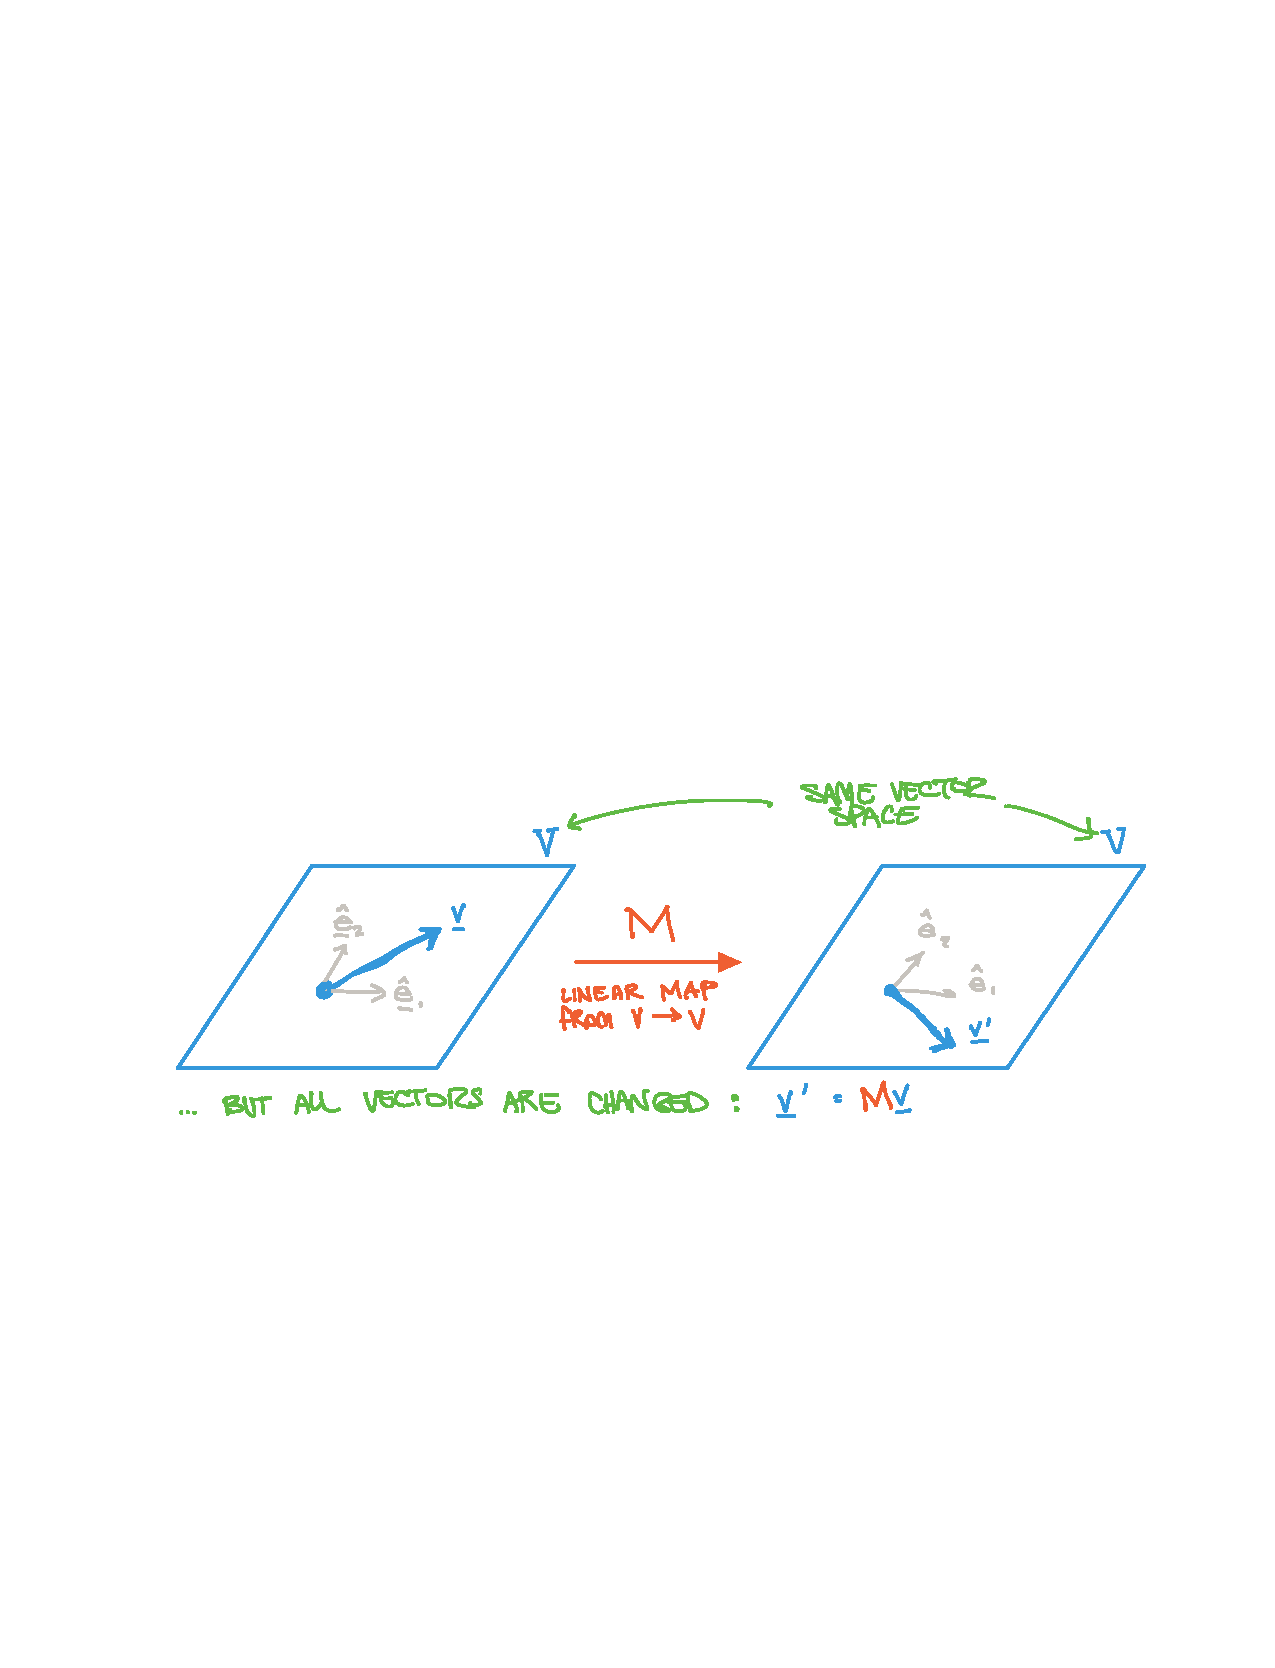
\includegraphics[width=\textwidth]{figures/lineartransformation.pdf}
    \caption{Example of a linear transformation. The transformation $M$ (for matrix) takes a vector $\vec{v}$ and turns it into a different vector that we call $\vec{v}'$. This new vector is related to $\vec{v}$ by the matrix $\vec{v'}=M\vec{v}$. \emph{Every} vector is transformed under the map $M$. This is an \emph{active transformation} where all vectors transform, but the basis (${\bas{e}}_i$) stays fixed.}
    \label{fig:Linear Transformation}
\end{figure}



\subsection{Linear transformations}


A function $f$ is \textbf{linear} if it satisfies:
\begin{align}
  f(\alpha x) &= \alpha f(x)
  &
  f(x+y) &= f(x) + f(y) \ .
  \label{eq:def:pre:linear}
\end{align}
Here $\alpha$ is a number, and $x$ and $y$ are some objects (perhaps vectors) on which the function has been defined to act. We may combine these two properties to write the condition of linearity in equation:
\begin{align}
  f(\alpha x + \beta y) = \alpha f(x)+\beta f(y)
  \label{eq:def:linear}
\end{align}
\begin{exercise}
Show that equations \eqref{eq:def:pre:linear} and \eqref{eq:def:linear} imply one another. Going from \eqref{eq:def:pre:linear} to \eqref{eq:def:linear} is slightly more tricky than the other way around.
\end{exercise}


\subsection{Linear Transformations in One Dimension}

The definition of `linear' has \emph{nothing to do with lines}. It is true that $y=mx+b$ is the equation for a line in the $(x,y)$ plane. This is not the same as $f(x)=mx+b$ being linear. In fact, $f(x)=mx+b$ is \emph{not} linear as a transformation of numbers, $\mathbbm{R}\to\mathbbm{R}$
\begin{exercise}
Show that $f(x) = mx+b$ does \emph{not} satisfy the definition of linearity, \eqref{eq:def:linear}. It is sufficient, for example, to consider $f(2x) \stackrel{?}{=}f(x)+f(x)$. Another cute way to see this is to consider linear combinations with zero, say $f(x+0)$.
\end{exercise}

\begin{exercise}
Show that $f(x) = mx$ is linear.
\end{exercise}

The problem in $f(x)=mx+b$ is the shift by a constant, $b$. I will comment that we can make up mathematics where `shift by a constant' is allowed. This, however, is no longer \emph{linear algebra}. You can look up affine spaces\footnote{\url{https://en.wikipedia.org/wiki/Affine_space}} if are curious. I only mention it here because the word `affine' may show up later in your mathematical physics studies---I want you to remember that it has something to do with constant shifts. 

\subsection{Linear Transformations in Two and Three Dimensions}

In Section~\ref{sec:index:notation} we introduced the idea that a matrix, $M$ has a peculiar index notation $M\aij{i}{j}$. This turned out to be convenient because we could use Einstein summation convention to conveniently write out what happens when we apply a matrix $M$ to a vector $\vec{v}$. You end up with a vector $M\vec{v}$ with components
\begin{align}
    (Mv)^i = M\aij{i}{j}v^j \ .
\end{align}
We recognized that the $j$ indices are \emph{contracted}. From an index point of view, these contracted indices ``cancel out'' so the resulting expression  only has one free index.\footnote{I say \emph{free} index to contrast it from a contracted (repeated) index that is summed over. We can put any allowed value into a free index and the equation is true.} This is good, the left-hand side of the above equation has one free index, so the right-hand side should also have exactly one free index.\footnote{This should remind you of dimensional analysis. If you have different dimensions on two sides of an equation, you have done something wrong.}




\subsection{The trivial transformation: identity matrix}

The identity matrix, $\mathbbm{1}$ leaves vectors unchanged: $\mathbbm{1}\vec{v} = \vec{v}$. You already know its components in $\mathbbm{R}^3$:
\begin{align}
    \mathbbm{1} = 
    \begin{pmatrix}
        1 & 0 & 0 \\
        0 & 1 & 0 \\
        0 & 0 & 1
    \end{pmatrix} \ .
\end{align}
Sometimes we will indicate the dimension of the space by writing $\mathbbm{1}_3$ or $\mathbbm{1}_{3\times 3}$ when we want to be extra clear. There is a useful way of writing the components of the identity matrix. Define the \textbf{Kronecker}~$\delta$: 
\begin{align}
    \delta^i_j &= 
    \begin{cases}
    1 & \text{ if }\, i=j\\
    0 & \text{ if }\, i\neq j
    \end{cases} \ .
\end{align}
Then we say that the components of $\mathbbm{1}$ are $\delta^i_j$, no matter what dimension of space we are in.

\emph{But wait}, you object, \emph{the indices are all messed up!} You are right. The indices on $\delta^{i}_j$ look wrong because we made a big deal that matrices have a first index and a second index that we must distinguish between. The first index is written upper, and the second index is lower. So should we not have written $\delta\aij{i}{j}$, with the $j$ clearly to the right of the $i$? 

Yes, this is technically correct. The reason why we made a big deal about this and wrote $M\aij{i}{j}$ instead of $M^i_j$ is that we will eventually want to consider alternative configurations of indices. For example, $T_{ij}$ or $S_i^{\phantom{i}j}$ or even weirder things like $R^\mu_{\phantom{\mu}\nu\rho\sigma}$.  It turns out that for the identity matrix, there is no ambiguity because
\begin{align}
    \delta^i_j = \delta\aij{i}{j} = \delta_i^{\phantom{i}j} .
\end{align}
So for convenience, we will just write $\delta^i_j$. Observe, however, that we \emph{never} write $\delta_{ij}$. There is no problem defining $\delta_{ij}$ in the same way, but it turns out that this combination rarely shows up.\footnote{Instead, there is a different mathematical structure called the metric, $g_{ij}$ that has two lower indices. Sometimes the metric components may be equal to the Kronecker $\delta$, so we may say $g_{ij}$ = $\delta_{ij}$. But in those cases we need to be clear that we are using the metric that happens to be the identity, not that we are multiplying by the identity. Why the big deal? One example is that the metric is where gravity lives---so it would be a rather big omission if we mistook it for ``multiplying by one.''}

It is useful to think about the Kronecker~$\delta$ as a machine that converts indices. Consider what it does to a vector:
\begin{align}
    (\mathbbm{1}\vec{v})^i = \delta^i_j v^j = 
    \delta^i_1v^1 + \delta^i_2v^2 + \delta^i_3v^3 \ .
\end{align}
On the right-hand side, there is exactly one non-zero term because $\delta^i_j$ is zero for all terms except when $j=i$. That means 
\begin{align}
    \delta^i_j v^j = v^i \ .
\end{align}
The right-hand side is, of course, what we expected since $\mathbbm{1}\vec{v} = \vec{v}$. So we can train ourselves to ``mechanically'' interpret the $\delta^i_j$ object as one that replaces indices. 
\begin{exercise}
Show that this works for lower indices as well. Consider the multiplication of two matrices, $M\mathbbm{1}$. Show that
\begin{align}
    M\aij{i}{j}\delta^j_k = M\aij{i}{k} \ ,
\end{align}
so that the $\delta^j_k$ simply replaces the $j$ index on $M\aij{i}{j}$ and turns it into a $k$.
\end{exercise}
\begin{exercise}
Even though we have not introduced any objects with more complicated index structure, suppose you have the following object: 
\begin{align}
    R^\mu_{\phantom{\mu}\nu\rho\sigma} \ .
\end{align}
The Greek letters are indices (like $i$ and $j$), we have switched notation because this is the convention for spacetime. An object with this index structure shows up in general relativity, it is called the Riemann tensor. Without knowing any general relativity, write out the value of
\begin{align}
    \delta^\mu_\alpha\,
    \delta^\nu_\beta\,
    \delta^\rho_\gamma\,
    \delta^\sigma_\tau\,
    R^\mu_{\phantom{\mu}\nu\rho\sigma} \ .
\end{align}
This is some kind of `matrix multiplication' by `identity matrices' hitting a $N\times N\times N\times N$ array of numbers, where $N=4$ is the dimension of spacetime. 
\end{exercise}

\subsection{Composition of linear transformations}

Suppose you have two linear transformations from $V\to V$, call them $f(\vec{x})$ and $g(x)$. These are represented by matrices $M$ and $N$, repectively. Then the \textbf{composition} of these two linear transformations is
\begin{align}
    f\circ g(\vec{x}) &\equiv f\left(g(\vec{x})\right)
    &
    \Leftrightarrow
    &
    f\circ g(\vec{x})&=
    MN\vec{x}
\end{align}
On the right-hand side we have written the matrix that represents $f\circ g$ as the product of the matrices for $f$ and $g$: $MN$. Matrix multiplication follows the usual rules. We can write this using summation convention very nicely. The matrices have components and index structure $M\aij{i}{j}$ and $N\aij{i}{j}$ respectively. Each has an upper index and a lower index. The product $MN$ has components
\begin{align}
    (MN)\aij{i}{j} = M\aij{i}{k}N\aij{k}{j} \ .
    \label{eq:matrix:multiplication}
\end{align}

\begin{example}
One thing that we notice from \eqref{eq:matrix:multiplication} is that the index structure makes it clear that the order of matrix multiplication matters.
\begin{align}
    (MN)\aij{i}{j} = M\aij{i}{k}N\aij{k}{j} 
    \neq 
    N\aij{i}{k}M\aij{k}{j} 
    =
    (NM)\aij{i}{j} \ .
\end{align}
Thus the order in which two linear transformations are composed matters. On the other hand, the order in which components (which are just numbers) are multiplied does not matter. For example:
\begin{align}
    (MN)\aij{i}{j} 
    = M\aij{i}{k} N\aij{k}{j}  
    = N\aij{k}{j} M\aij{i}{k} \ .
\end{align}
The sums on the right-hand side both represent the same series of terms. Neither of those sums are the same as 
\begin{align}
    (NM)\aij{i}{j}
    =
    N\aij{i}{k}M\aij{k}{j}
    =
    M\aij{k}{j} N\aij{i}{k} \ .
\end{align}
This is the kind of manipulation that is pretty obvious at its core, but the first time you see this manipulation done in textbook it can be pretty disorienting. 
\end{example}
The above example makes the following point clear: The order in which components are multiplied is \emph{not} the same as the order in which the linear transformations are applied. That is, the order of the components are multiplied not the same as the order in which the matrices are multiplied.
\begin{example}
If you want to recover the ``matrix multiplication'' $MN$ from the ``component contraction'' $M\aij{i}{k} N\aij{k}{j}  
    = N\aij{k}{j} M\aij{i}{k}$, you should start by writing out the terms so that neighboring indices are contracted. The expression $M\aij{i}{k} N\aij{k}{j}$ has neighboring $k$ indices contracted, while the equivalent expression $N\aij{k}{j} M\aij{i}{k}$ does not. Thus we take $M\aij{i}{k} N\aij{k}{j}$ and then we can ``promote'' this back to a matrix multiplication, $MN$. A caveat: physicists often prefer to work with component contractions instead of matrix multiplications. In fact, with more complicated tensor contractions, it is not always meaningful or possible to recover a ``matrix multiplication'' form.
\end{example}


\begin{exercise}\label{ex:product:of:diagonal:matrices}
A \textbf{diagonal matrix} is one where the only non-zero components are along the diagonal. We will sometimes write diagonal matrices with a hat, $\hat M$, to indicate that they are diagonal. Sometimes we abbreviate the definition of a diagonal matrix by only specifying its diagonal components:
\begin{align}
    \hat M = 
    \begin{pmatrix}
        2 & 0 & 0 \\
        0 & 7 & 0 \\
        0 & 0 & 4  
    \end{pmatrix}
    =
    \text{diag}(2,7,4) \ .
\end{align}
Show that the product of diagonal matrices is also diagonal whose components are the products of the diagonal components. You can use \eqref{eq:matrix:multiplication} armed with the knowledge that $(\hat M)\aij{i}{j} = 0$ if $i\neq j$. Then you must show that $(\hat M \hat N)\aij{i}{j} = 0$ for $i\neq j$. Finally, check the values of the diagonal elements to show that
\begin{align}
    \hat M \hat N = \text{diag}\left(M\aij11 N\aij11 \;,\;\, M\aij22 N\aij 22 \;,\;\, M\aij33 N\aij 33\right) \ .
\end{align}

\end{exercise}


\subsection{Linearity and Basis Vectors}

\paragraph{A couple of useful exercises}
Here's a pair of exercises that are worth trying out:
\begin{exercise}
Calculate the following linear transformations by a matrix $M$ on two different vectors, $\vec{v}$ and $\vec{w}$:
\begin{align}
    M\vec{v} &= 
    \begin{pmatrix}
        \pp 3 & 2 & \pp 1 \\
        - 1 & 4 & -2 \\
        \pp 0 & 1 & \pp 1
    \end{pmatrix}
    \begin{pmatrix}
        2 \\ 1 \\ 1
    \end{pmatrix}
    = \quad ?
    &
    M\vec{w} &= 
    \begin{pmatrix}
        \pp 3 & 2 & \pp 1 \\
        - 1 & 4 & -2 \\
        \pp 0 & 1 & \pp 1
    \end{pmatrix}
    \begin{pmatrix}
        -1 \\ \pp 0 \\ 3
    \end{pmatrix}
    = \quad ?
\end{align}
\end{exercise}
\begin{exercise}
That was tedious, wasn't it? What if I asked you to calculate three more...
\begin{align}
    M
    \begin{pmatrix}
        1 \\ 1 \\ 4
    \end{pmatrix}
    &= \quad ?
    &
    M
    \begin{pmatrix}
        0 \\ 1 \\ 7
    \end{pmatrix}
    &= \quad ?
    &
    M
    \begin{pmatrix}
        \pp 3 \\ \pp 1 \\ -2
    \end{pmatrix}
    &= \quad ?
    \label{eq:eg:more:multiplications}
\end{align}
\end{exercise}
Did you do it? Go ahead, do these calculations. Use \emph{Mathematica} if you must. Did you do it the hard way, or did you notice that there's an easy way? 

\paragraph{General two-dimensional discussion}
The easy observation is that each of the vectors being acted on in \eqref{eq:eg:more:multiplications} are \textbf{linear combinations} of $\vec{v}$ and $\vec{w}$. What you should notice is that
\begin{align}
    \begin{pmatrix}
        1 \\ 1 \\ 4
    \end{pmatrix}
    = \vec{v} + \vec{w}
    &
    & 
    M
    \begin{pmatrix}
        1 \\ 1 \\ 4
    \end{pmatrix}
    &=
    M(\vec{v} + \vec{w})
    = M\vec{v} + M\vec{w} \ .
\end{align}
In other words: if $\vec{u} = \vec{v} + \vec{w}$ and we already know the action of a matrix $M$ on $\vec{v}$ and $\vec{w}$---that is, we know $M\vec{v}$ and $M\vec{w}$---then we're basically done. No further matrix multiplication is needed! We can simply use the linearity of $M$ to take a linear combination of $M\vec{v}$ and $M\vec{w}$. You should check that this is true for the other matrix multiplications in \eqref{eq:eg:more:multiplications}.


This is a big deal. We know that $\vec{v}$ and $\vec{w}$ are the \textbf{basis vectors} for a subspace $V_2 = \text{Span}(\vec{v},\vec{w})$. We have established that if we know the action of $M$ on the basis vectors of $V_2$, then we know the action of $M$ on any vector in $V_2$. This is because any vector in $V_2$ has the form
\begin{align}
    \vec{u} = a\vec{v} + b \vec{w}
\end{align}
for two numbers $a$ and $b$. Then the action of $M$ on any such vector is
\begin{align}
    M\vec{u} = a(M\vec{v}) + b(M\vec{w}) \ .
    \label{eq:Mu:aMv:bMw}
\end{align}

We can pose this in the following way. Suppose we have a two-dimensional vector space $V_2$
 with some basis $\vec{b}_1$ and $\vec{b}_2$. Now suppose we have a linear transformation $M$ that goes from $V_2\to V_2$. This is a matrix. 
\begin{enumerate}
    \item We know that the matrix is encoded by $2\times 2= 4$ numbers, each of the four elements, $M\aij{i}{j}$. If you know these four elements, then you can matrix multiply any vector in $V_2$ by simply using the matrix multiplication rules. All you need to specify is the vector $\vec{u}$, which is encoded by its two components $u^i$. Then you get two numbers as output, $(Mu)^i = M\aij{i}{j}u^j$.
    \item Alternatively, we suppose that we do not know (or we deliberately forget) the four elements $M\aij{i}{j}$. Instead, suppose we know the components of $M\vec{v}$ and $M\vec{w}$. These are each two component vectors, so this is a total of four numbers. Then we may specify $\vec{u}$ not by its components $u^i$, by its coefficients $a$ and $b$. Then we may use \eqref{eq:Mu:aMv:bMw} to specify the two components of $M\vec{u}$.
\end{enumerate}
In each picture, you specify the four numbers that encode the transformation and then use them to calculate the action of $M$ on a generic vector $\vec{u}$. 

\begin{example}
The two approaches above are equivalent when the basis vectors are
\begin{align}
    \vec{b}_1 = {\bas{e}}_1 &= \begin{pmatrix}
        1 \\ 0
    \end{pmatrix}
    &
    \vec{b}_2 = {\bas{e}}_2 &= \begin{pmatrix}
        0 \\ 1
    \end{pmatrix}\ .
\end{align}
This should be clear since
\begin{align}
    M {\bas{e}}_1 &= 
    \begin{pmatrix}
        M\aij{1}{1} \\ M\aij{2}{1}
    \end{pmatrix}
    &
    M {\bas{e}}_2 &= 
    \begin{pmatrix}
        M\aij{1}{2} \\ M\aij{2}{2}
    \end{pmatrix} \ .
    \label{vec:Mhate:2}
\end{align}
\end{example}
The example above tells us that the `components of a matrix' have a specific meaning: they encode the action of $M$ on a particularly nice basis, ${\bas{e}}_{1,2}$. This is significant for the following reason: while a matrix may encode a linear transformation, we should not be settle into thinking that the $2\times 2$ of numbers somehow \emph{is} the matrix.
\begin{example}
$M\aij 11$ is simply the coefficient of ${\bas{e}}_1$ in the expansion of $M{\bas{e}}_1$. $M\aij 12$ is simply the coefficient of ${\bas{e}}_2$ in the expansion of $M{\bas{e}}_1$. 
\end{example}



 

\paragraph{General discussion}
The general version of this discussion is as follows. We write $\mathbbm{R}^N$ to be $N$-dimensional real space. A linear transformation from $\mathbbm{R}^N \to \mathbbm{R}^N$ is a matrix. Suppose we have a nice basis. In fact, the `obvious' basis is
\begin{align}
    {\bas{e}}_1 &= 
    \begin{pmatrix}
        1 \\ 0 \\ 0 \\ \vdots
    \end{pmatrix}
    &
    {\bas{e}}_2 &= 
    \begin{pmatrix}
        0 \\ 1 \\ 0 \\ \vdots
    \end{pmatrix}
    &
    \cdots &
    &
    {\bas{e}}_N &= 
    \begin{pmatrix}
        0 \\ \vdots \\ 0 \\ 1
    \end{pmatrix} \ .
\end{align}
Then we know that any vector in $\mathbbm{R}^N$ may be written as a linear combination of these basis vectors. In fact, this is \emph{precisely} what we mean by the components of a vector: it is the coefficient of each ${\bas{e}}_i$ basis vector in the linear combination that represents the vector:
\begin{align}
    \vec{v} &= v^i{\bas{e}}_i 
    &
    \vec{v} &\;\text{``=''}\;
         \begin{pmatrix}
        v^1 \\ v^2 \\ \vdots \\ v^N
    \end{pmatrix} \ .
\end{align}
The first equality is \emph{true}. It defines the meaning of $v^i$ no matter what the ${\bas{e}}_i$ are, whether they are columns or more abstract objects. The equation on the right has air quotes because it is not really an equation. What it means is $\vec{v}$ \emph{is represented by the following column of numbers}. The column of numbers simply mean the coefficients of the basis vectors---no matter what the basis vectors are.


In physics, we treat lots of different things as vectors. Momenta, electric fields, wavefunctions, and so forth. When we say that the electric field at a point is a vector, we do not mean that there is actually an invisible arrow with some length and direction there. Nor do we mean that the electric field at that point is a column of three numbers. What we mean is that these three numbers represent the components of the electric field with respect to a basis. The basis are usually the electric field in the $x$, $y$, and $z$ directions. 


If we know the action of $M$ on the basis vectors, what that really means is that we know the components of $M{\bas{e}}_i$ for each $i$. That is to say, 
\begin{align}
    M{\bas{e}}_i &= (M{\bas{e}}_i)^k {\bas{e}}_k 
    &
    M\aij{k}{i} &\equiv (M{\bas{e}}_i)^k
    \ .
\end{align}
Be very careful with this. What we mean is the $N$-dimensional generalization of \eqref{vec:Mhate:2}, so refer back to that if the notation is cumbersome. What is important here is that we now have a definition of the components $M\aij{i}{j}$ that is fully general. 



\subsection{Linear transformations as maps acting on basis vectors}

The relation between the components of linear transformations and basis vectors is elucidated in Fig.~\ref{fig:map:M}. A vector is a linear combination of the basis vectors, so the action of a linear transformation $M$ on a vector $\vec{v}$ reduces to taking linear combinations of the action of $M$ on the basis vectors $\bas{e}_i$:
\begin{align}
    \vec{v} &= v^i\bas{e}_i 
    M\vec{v} &= v^i\, M\bas{e}_i 
    \ .
    \label{eq:v:Mv:basis:action}
\end{align}
There are several observations:
\begin{itemize}
    \item We could define a basis $\vec{f}_i \equiv M\bas{e}_i$. Then the components of $\vec{v}$ in the $\bas{e}_i$ basis are the same as the components of $M\vec{v}$ in the $\vec{f}_i$ basis. 
    \item The components of $M\vec{v}$ in the $\bas{e}_i$ basis are \emph{not} the $v^i$, but rather the linear combinations $M\aij{i}{j}v^j$. We know this from our matrix multiplication rules, but we can also see it from the linear combination $v^i\, M\bas{e}_i$ and the observation that the matrix components $M\aij{i}{j}$ are simply the components of $M\bas{e}_i$, as we saw in \eqref{vec:Mhate:2}.
    \item What is nice about \eqref{eq:v:Mv:basis:action} is that we have separated the \emph{components} of a vector $v^i$ from the ``vector-y'' part, $M\bas{e}_i$. What we mean by this is that the \emph{components} are just numbers. They are coefficients of a linear combination and are what we write as the components of a column of numbers. However, vectors are not always ``columns of numbers.'' We want to abstract what a vector is and thus we need to also abstract what a linear transformation is. All of that abstraction is encoded in the basis vectors and the definition of the transformation acting on the basis vectors. 
\end{itemize}


\begin{figure}[tb]
    \centering
    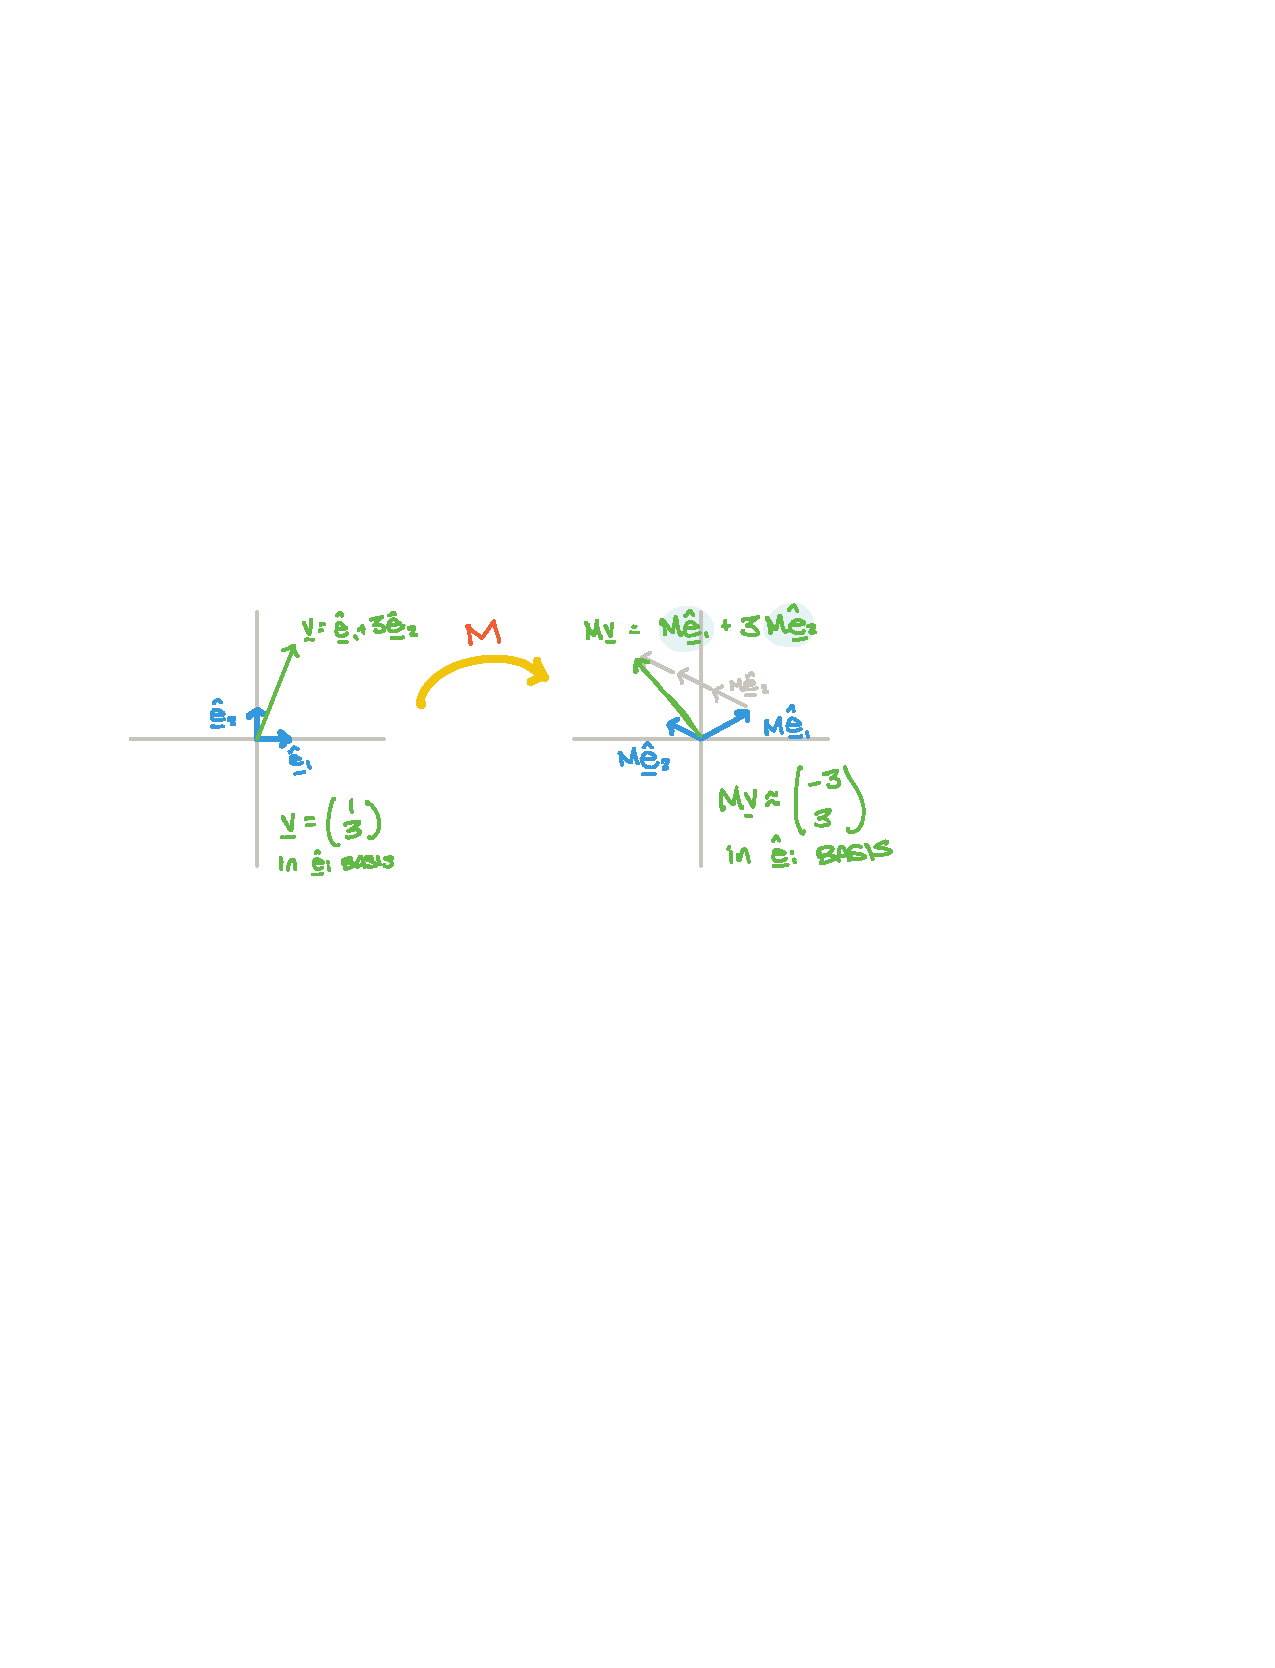
\includegraphics[width=.8\textwidth]{figures/maps_M.pdf}
    \caption{$M$ is a linear transformation from $\mathbbm{R}^2\to\mathbbm{R}^2$. If we know the action of $M$ on the basis vectors $\bas{e}_i$ of $\mathbbm{R}^2$, then we know the action of $M$ on any vector $\vec{v}$.}
    \label{fig:map:M}
\end{figure}




\subsection{Inverse transformations}

% Pre-image, image, kernel, 
% Non-invertible

Let $M$ be a linear transformation from $V\to V$. This is just to say that $M$ is a matrix that acts on vectors in $V$. For ``nice'' matrices, $M$, there is a unique \textbf{inverse} matrix (inverse transformation) $M^{-1}$ with components $(M^{-1})\aij{i}{j}$. The defining property of the matrix inverse is $M^{-1}M = \mathbbm{1}$. That means that $M^{-1}(M\vec{v})=\vec{v}$ for any vector $\vec{v}$. The matrix inverse simply undoes the transformation $M$. This is shown in Fig.~\ref{fig:map:M:inv}. 

% \flip{in progress}
% not always defined.


\begin{figure}[tb]
    \centering
    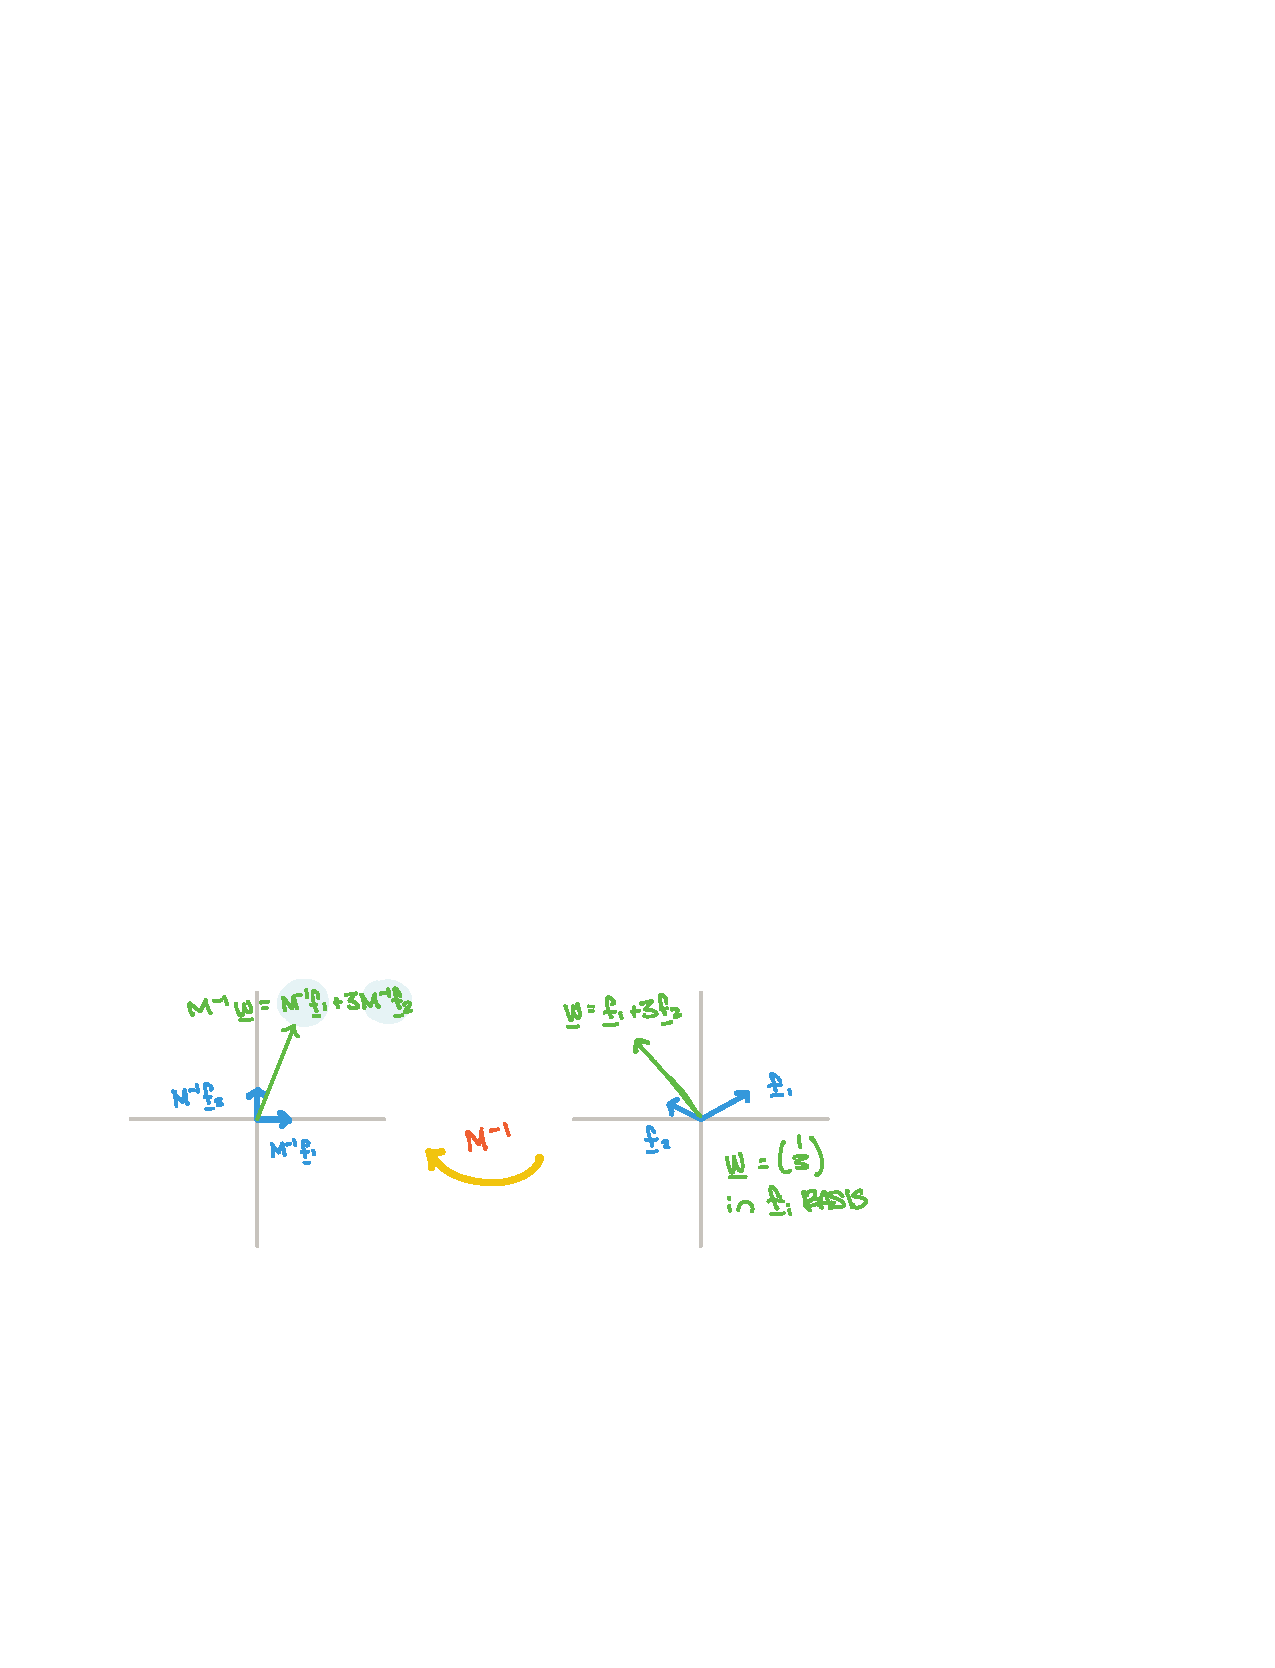
\includegraphics[width=.8\textwidth]{figures/maps_Minv.pdf}
    \caption{Let $M$ is a linear transformation from $\mathbbm{R}^2 \to \mathbbm{R}^2$, as we drew in Fig.~\ref{fig:map:M}. Now assume that you have a vector $\vec{w}$ that is the linear combination of some basis vectors $\vec{f}_i$, see the right-hand side of the sketch. If the $\vec{f}_i$ can be obtained as the transformation by $M$ of some other vectors---the basis vectors we called $\bas{e}_i$ in Fig.~\ref{fig:map:M}---then the inverse transformation $M^{-1}$ acts as a map ``back'' to the original basis. }
    \label{fig:map:M:inv}
\end{figure}

Given a basis, matrices are described by their components, $M\aij{i}{j}$. How do you find the components of the inverse matrix, $(M^{-1})\aij{i}{j}$? The most straightforward way is the hard way. Let us consider the $2\times 2$ case. We know that the defining relationship is
\begin{align}
    M(M^{-1})=(M^{-1})M &= \mathbbm{1}
    &
    M\aij{i}{k}(M^{-1})\aij{k}{j}
    =
    (M^{-1})\aij{i}{k}M\aij{k}{j} 
    = \delta^i_j \ .
    \label{eq:inverse:matrix:definition}
\end{align}
On the right we have four equations for each combination of $i,j \in\{1,2\}$. We also have four unknown components, $(M^{-1})\aij{i}{j}$. This is a system of linear equations that one can usually solve. Sometimes the system will not be solvable---in that case the matrix $M$ is not invertible.

\begin{exercise}
Convince yourself that \eqref{eq:inverse:matrix:definition} holds for \emph{any} vector space of any dimension, $N$. You end up with $N^2$ equations for $N^2$ unknown components $M\aij{i}{j}$. Does this change if all of the components are allowed to be complex numbers?
\end{exercise}

\begin{example}
The inverse of a diagonal matrix is easy:
\begin{align}
    M &=
    \begin{pmatrix}
     3 & \pp  0 \\
     0 & -2
    \end{pmatrix}
    &
    M^{-1} &=
    \begin{pmatrix}
    \frac{1}{3} & \pp 0 \\
    0 & -\frac{1}{2}
    \end{pmatrix} \ .
\end{align}
We have used the earlier observation in Exercise~\ref{ex:product:of:diagonal:matrices} that the product of diagonal matrices $\hat M$ and $\hat N$ is also a diagonal matrix whose elements are the products of the corresponding elements in $\hat M$ and $\hat N$.
\end{example}

Physical states are often described by vectors. The dynamics of a theory of physics are then described by linear transformations of vectors. Usually this is some description of the change in the vector over some infinitesimal time. This change is a response to some source of the dynamics. You end up with formulas that always look like
\begin{align}
    M \vec{v} &= \vec{s} 
    &
    \Leftrightarrow
    &
    (\text{dynamics})(\text{state}) = (\text{source}) \ .
\end{align}
The source is something like a pebble falling into a pond. The dynamics are a matrix that describes how ripples propagate. The state is the configuration of the water in the pond.
%
The problem that you have to solve in physics is usually framed as follows: If you are given some source $\vec{s}$, what is the value of the state $\vec{v}$? This requires taking the inverse of the dynamics $M$. 

Thus far we have seen two things: first, finding the components of an inverse matrix is generally very annoying. Secondly, there is at least one case---when the matrix is diagonal---where the annoying task is significantly simplified. It turns out that there are more clever ways to invert a matrix that often apply for the types of matrices that show up in physics. These tricks boil down to converting matrices into their diagonal form.



\subsection{Matrices that aren't invertible: Projections}

Solving for the components of a matrix inverse boils down to $N^2$ equations for $N^2$ unknowns. This does not mean that those equations have a solution. A simple example is the case of a diagonal matrix with one component zero. We illustrate this in Fig.~\ref{fig:map:M:no:inv}
\begin{figure}[tb]
    \centering
    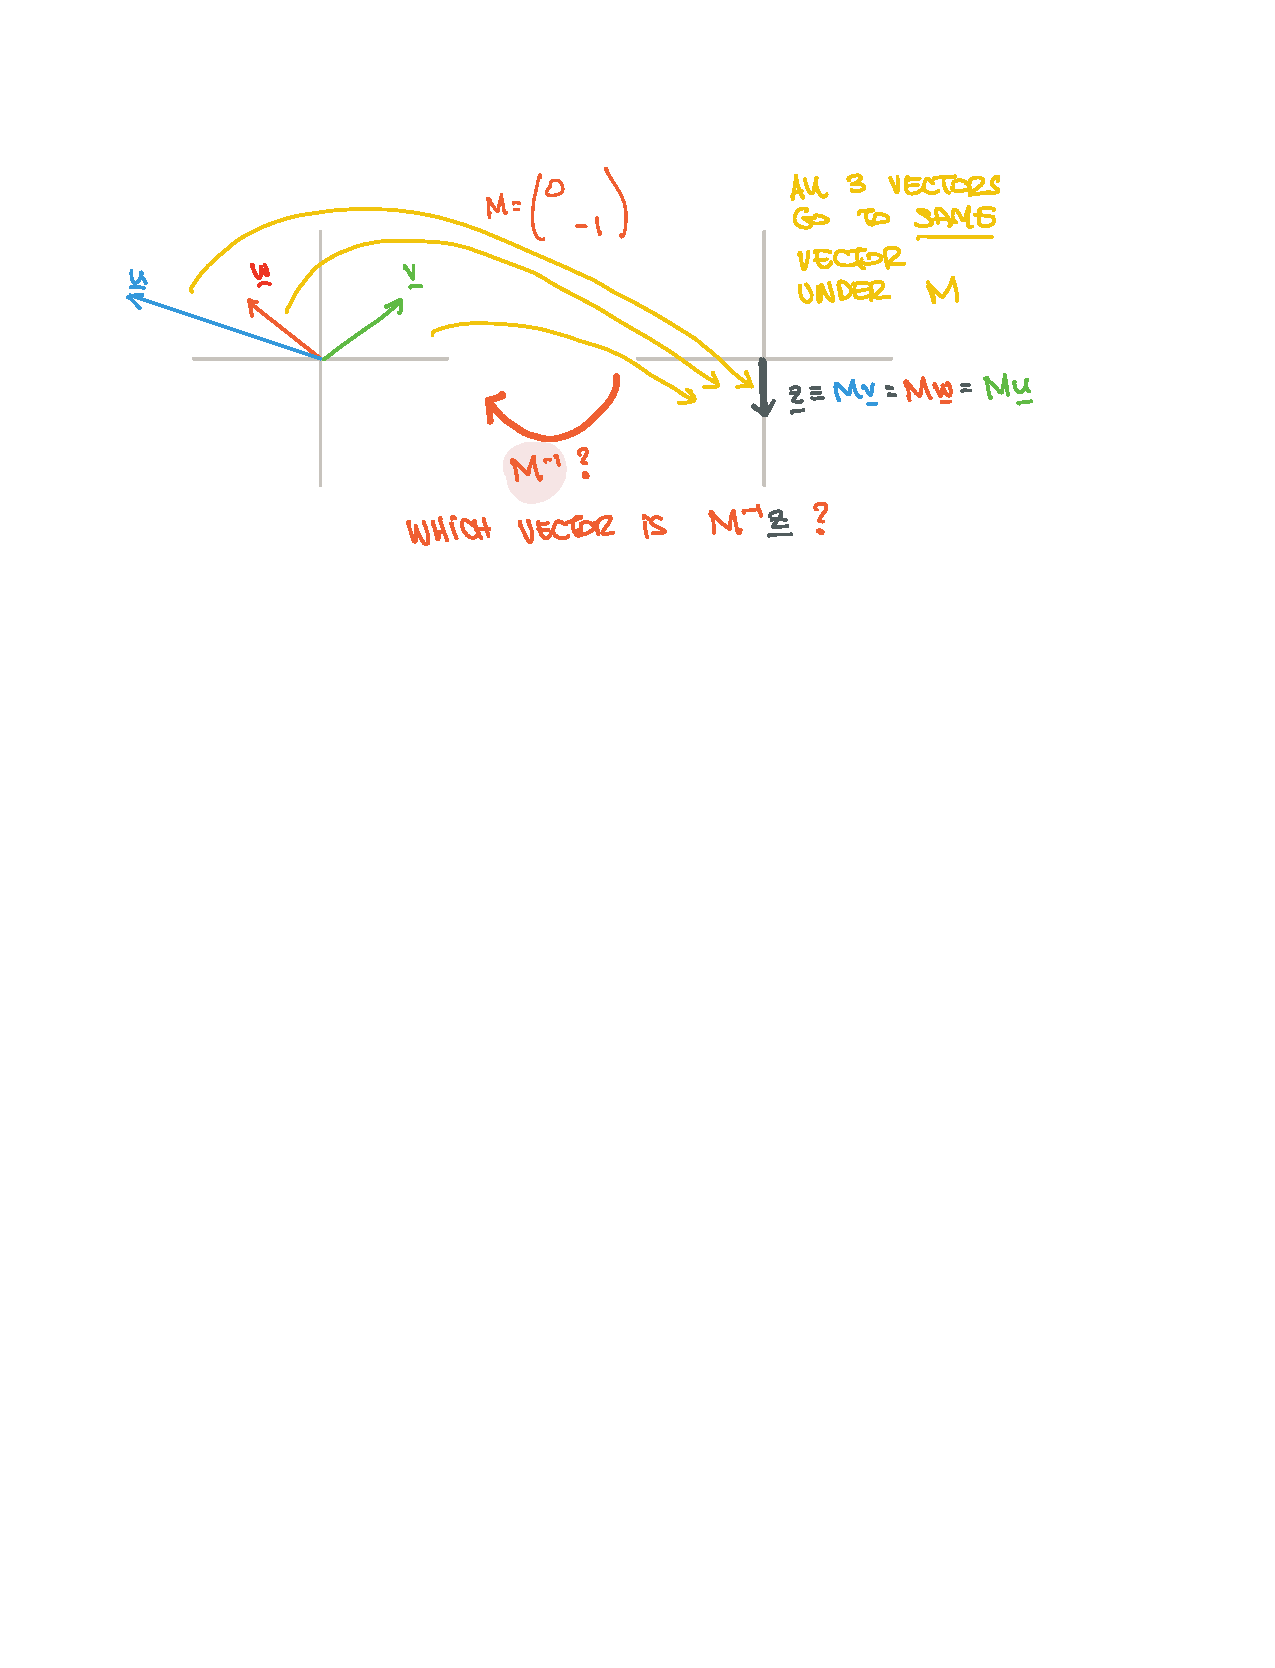
\includegraphics[width=.8\textwidth]{figures/maps_noninv.pdf}
    \caption{$M$ is a non-invertible matrix. We notice that there's no problem applying $M$ to vectors. The odd thing is that there are multiple vectors---$\vec{v}$, $\vec{w}$, and $\vec{u}$ in the picture---that all turn into the same vector, $M\vec{v} = M\vec{w}=M\vec{u}\equiv \vec{z}$. The problem shows up when we try to ``undo'' the transformation $M$ by applying $M^{-1}$ to $\vec{z}$. $M^{-1}\vec{z}$ should be a vector. Instead, we have at least three different valid options: $\vec{v}$, $\vec{w}$, and $\vec{u}$. This means that $M^{-1}$ is not a well defined linear map: it can send one vector $\vec{z}$ into many possible vectors. }
    \label{fig:map:M:no:inv}
\end{figure}
% 
Thinking of the matrix $M$ as a map, we see the the problem is one of uniqueness. A linear map should take each vector $\vec{v}$ into a single, well-defined vector $M\vec{v}$. $M$ is suspicious because it sends multiple different vectors to the \emph{same} vector, say $M\vec{v} = M\vec{w}$. That's fine. Each of $\vec{v}$ and $\vec{w}$ are sent to \emph{a} vector. The problem shows up when we try to take the inverse. If we write $\vec{z} = M\vec{v} = M\vec{w}$, we know that
\begin{align}
    (M^{-1})\vec{z} = (M^{-1})M\vec{v} &= \vec{v}
    &
    (M^{-1})\vec{z} = (M^{-1})M\vec{w} &= \vec{w} \ .
\end{align}
However, we assumed that $\vec{v} \neq \vec{w}$. This means makes the above line inconsistent. The inverse transformation is not defined. Bummer.

Fortunately, most of the \emph{dynamics} in physics \emph{is} invertible. That does not mean that we can ignore non-invertible matrices, though. Non-invertible matrices can be understood as \textbf{projections} onto a subspace. You can see this in the example in Fig.~\ref{fig:map:M:no:inv}. The map $M$ is essentially only using the information about the second component of its input vector and mapping it to just the second component of the output vector. That means that $M$ is really just a map to a one-dimensional subspace. In this way, the two dimensional vector space $\mathbbm{R}^2$ is \textbf{projected} onto a one-dimensional subspace of $\mathbbm{R}^2$. In that example, the one dimensional space is defined by vectors of the form
\begin{align}
    \vec{v} = 
    \begin{pmatrix}
    0\\ v^2    
    \end{pmatrix} \ .
\end{align}

Projections are really useful in physics. Sometimes you want to take a big vector space and only focus on a subspace that satisfy certain conditions. For example, it turns out that in nature you can have two types of massless matter particles: left-handed and right-handed according to their quantum spin in the direction of their motion. One may want to project onto only the space of left-handed particles because that is easier to deal with than the entire space. Because projections necessarily ``throw out'' information, they are non-invertible.\footnote{I think this was more intuitive to past generations of physicists. When you throw out a piece of paper, it ends up in a recycling plant and it gets torn up and is lost forever. Since the advent of computers, when you ``throw out'' a file, you can usually control/command-z and undo to bring it back.}

\begin{example}
One of the most curious puzzles in fundamental physics over the last half century is the black hole information paradox.\footnote{\url{https://www.quantamagazine.org/the-most-famous-paradox-in-physics-nears-its-end-20201029/}} One way of stating the paradox is the question of whether or not ``falling into a black hole'' is a \emph{projection} that throws out information. 
\end{example}

\subsection{Trace}

The \textbf{trace} of a matrix $M$ is simply the sum of its diagonal components:
\begin{align}
    \text{Tr}\,M = M\aij{i}{i} = M\aij{1}{1} + M\aij{2}{2} + \cdots \ .
\end{align}
It is not obviously meaningful from the perspective of $M$ being a linear transformation. However, it ends up being useful as as a mechanical procedure that one can do to matrices. The reason for this is something we will see soon: the trace of a matrix is unchanged under rotations. 

\subsection{Determinants}

Here's another seemingly strange operation that you can do on a matrix. The determinant of a $2\times 2$ matrix is defined to be
\begin{align}
    \det M \equiv M\aij11 M\aij12 - M\aij12 M\aij21 \ .
\end{align}
Weird, right? Determinants for higher-dimensional square matrices can be defined recursively by taking specific linear combinations of sub-matrices. There are silly rules for this. There are fancy words for the sub-matrices (minors) and the appropriate sign for summing together those determinants (cofactors). Look, it's a mess. You should be able to calculate the determinant of a general $2\times 2$ matrix because it's easy. In case of national crisis, you should be able to calculate the determinant of a general $3\times 3$ matrix after consulting a reference to double check the signs. However, at this stage we will not make a big deal about determinants. I think engineering classes make a big deal about determinants because they can help with solving systems of linear equations using matrices---but \emph{that's not the kind of linear algebra we're doing in physics}.

\begin{example}
The determinant of a diagonal matrix is simply the product of each of its diagonal elements. 
\end{example}

Determinants of a matrix are at least as curious as its trace because the determinant of a matrix turns out to also be unchanged under rotations. Furthermore, in multivariable calculus, the determinant shows up in the volume element. In fact, there is a formal definition of the determinant that comes from differential geometry where we use the determinant to rigorously define volumes of curved spaces. This sort of thing shows up in general relativity.




\subsection{Matrices that aren't square: maps between vector spaces}

You may be wondering why all of our linear transformations are square. After all, you have probably seen rectangular matrices where the number of rows does not equal the number of columns. For example
\begin{align}
    W = 
    \begin{pmatrix}
        1 & \pp 2 &-6 & 7 \\
        6 & -3 & \pp 3 & 0
    \end{pmatrix} \ .
\end{align}
Just by looking at this, you can tell that $W$ acts on some kind of vector with four components and outputs a vector with two components. Assuming these vectors are part of $\mathbbm{R}^4$ and $\mathbbm{R}^2$ respectively, this means that $W$ is a map from $\mathbbm{R}^4$ to $\mathbbm{R}^2$, or
\begin{align}
    W:\; \mathbbm{R}^4 \;\to \; \mathbbm{R}^2 \ .
\end{align}
Non-square matrices are maps between different vector spaces. In this course we will have very little to say about non-square matrices. The type of linear algebra that comes up over and over again in physics are transformations from some vector space $V$ to itself.\footnote{To be more technically precise: the maps tend to be between vector spaces $V$ and $V'$ that are isomorphic to one another, $V\cong V'$. This means that the vector spaces may be different, but there is a unambiguous translation between the two.} 

The one thing we have observed about non-square matrices is that the number of columns is the maximum dimensionality of the input space, and the number of rows is the maximum dimensionality of the output space.\footnote{Why do we specify `maxmimum'? You could imagine a vector space that is two dimensional but happens to be written in a silly way as three-component vectors. For example, we could consider the space of vectors spanned by the $x$- and $y$-basis vectors but written as three component vectors in $\mathbbm{R}^3$. That space is two dimensional, but the vectors have three components---one of which is always zero.} The dimensionality tells us about how much information is in a vector. A three-dimensional vector space has ``three numbers worth'' of information, the three components relative to a basis. This means that:
\begin{enumerate}
    \item If the number of columns is larger than the number of rows, then the output of the transformation may have less information than the input. For example, two different input vectors may map to the same output vector.
    \item If the number of rows is larger than the number of columns, then input of the transformation may not be able to encode enough information to populate every possible vector in the output space. For example, there may be vectors $\vec{v}_\text{out}$ in the output space that cannot be written as $W\vec{u}_\text{in}$. 
\end{enumerate}
There are some fancy words that are associated with these ideas. The \textbf{kernel}\footnote{The word kernel is really annoying here because it shows up in another place in the theory of distributions. Much to my chagrin, we will argue that distributions are an ingredient in the linear algebra of infinite dimensional vector spaces. This means that there is a place later in this course where the word \emph{kernel} will come up again but will mean something completely unrelated.} of a transformation $M$ is the set of all vectors $\vec{v}$ such that $M\vec{v} = 0$. The \textbf{image} of a transformation is the set of all vectors $\vec{v}$ that can be obtained by acting with the transformation $M$, that is: there is some $\vec{u}$ such that $\vec{v} = M\vec{u}$.
\begin{exercise}
Using the definition of a vector space, show that the kernel of $M$ and the image of $M$ are vector spaces. 
\end{exercise}

From this, we have argued that if $W: V_1 \to V_2$ is a linear transformation between two different vector spaces of different dimension, then 
\begin{enumerate}
    \item If the dimension of $V_1$, $\text{dim}\,V_1$, is larger than the dimension of $V_2$, $\text{dim}\,V_2$, then the kernel of $W$ contains more than just the zero vector.
    \item Alternatively, if $\text{dim}\,V_2 > \text{dim}\,V_1$, then the image of $W$ is a subspace of $V_2$ that does not contain all of $V_2$. 
\end{enumerate}

% \subsection{More Jargon}

\section{Rotations}

\subsection{Rotations in Two-Dimensions}

\subsection{Transformation of Vectors}

\subsection{Transformation of Row Vectors}

\subsection{Transformation of Matrices}

\subsection{Transformation of Tensors}

\subsection{Rotations in Three-Dimensions}

% non commutivity

\subsection{Invariance of Trace and Determinant}

\subsection{Exponentiation of Generators}

\subsection{Symmetry and Indices}

\subsection{Active versus Passive}
\begin{figure}[tb]
    \centering
    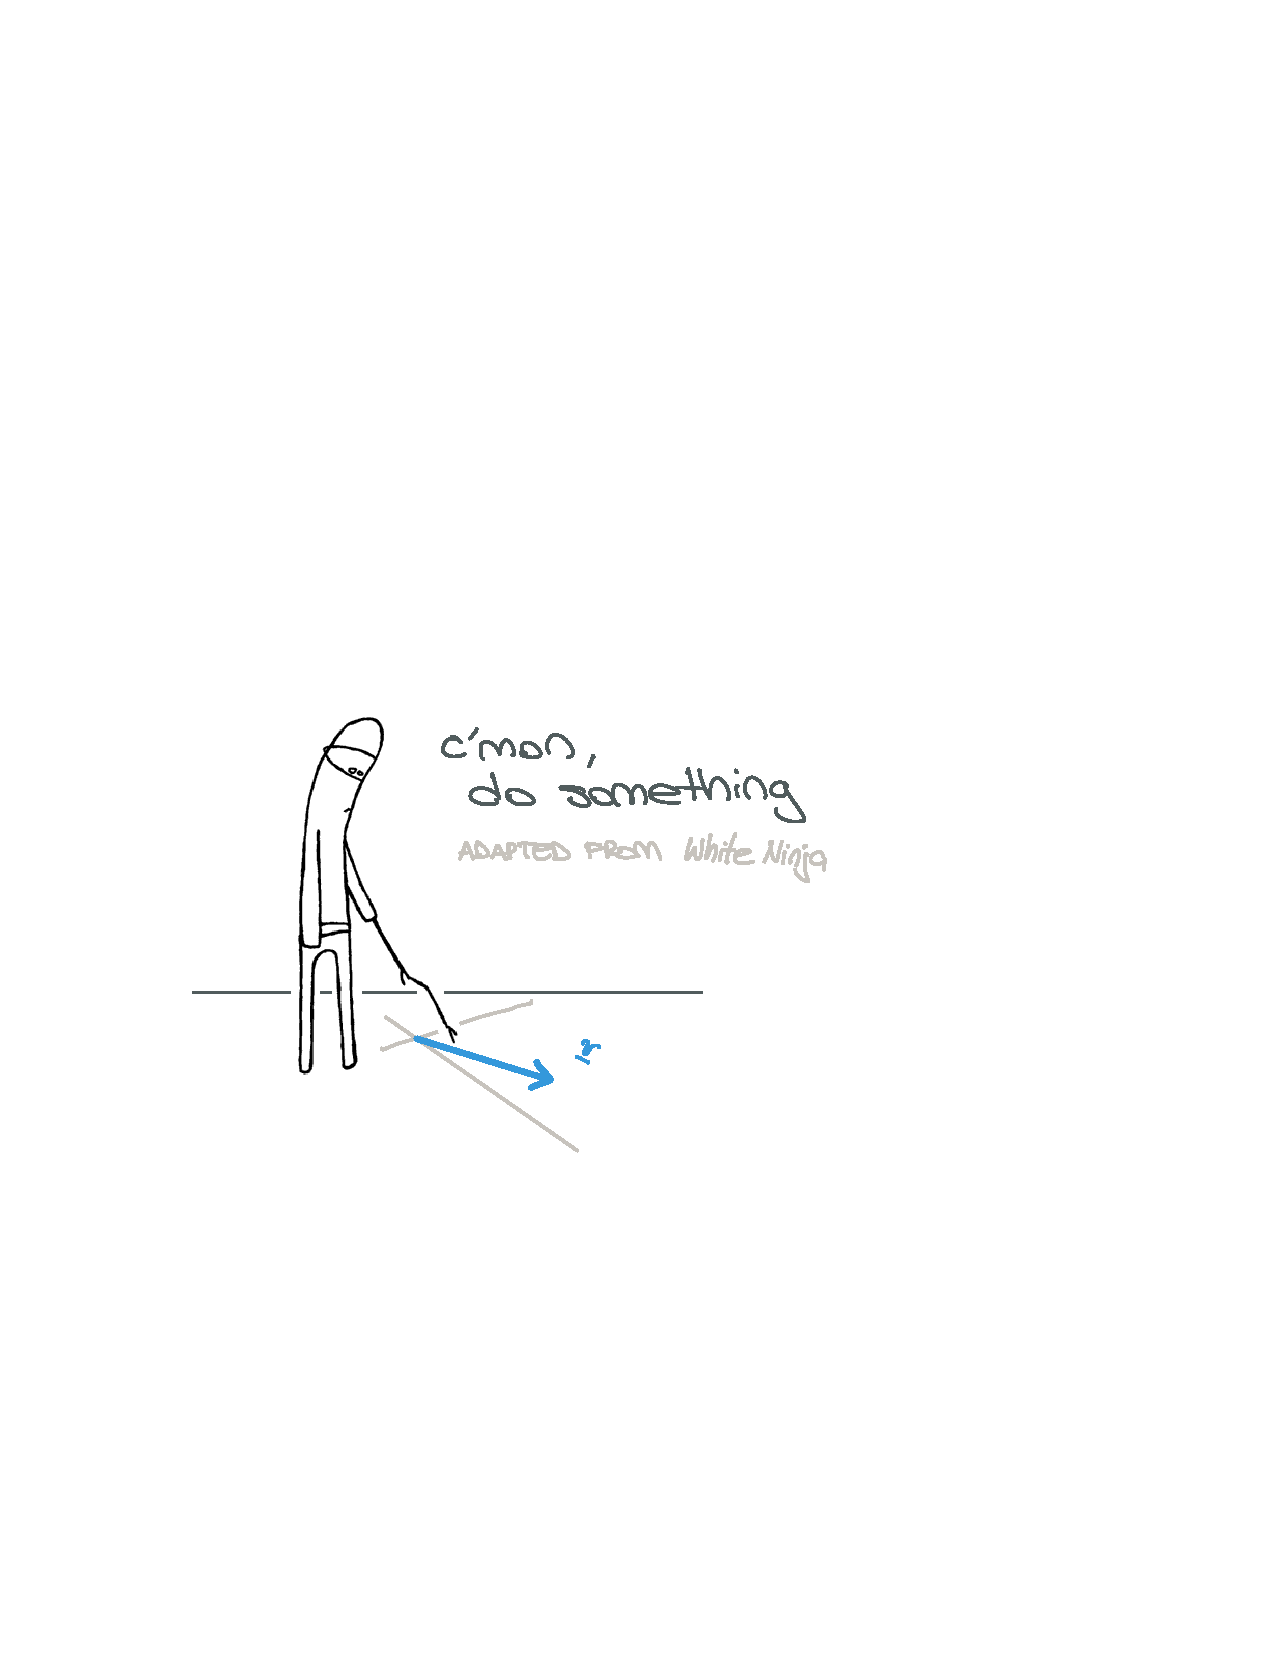
\includegraphics[width=.5\textwidth]{figures/passivetransform_dosomething.pdf}
    \caption{
        Nothing actually happens during a passive transformation. The basis vectors transform, but the components of the vector transform in such a way that $v'^i\bas{e}'_i = v^i\bas{e}_i$. Such a `transformation' may come off as uninspiring, but this is the basis of symmetries in physics. 
        From \url{https://knowyourmeme.com/memes/cmon-do-something}.
    }
    \label{fig:map:M}
\end{figure}



Passive is a symmetry. Active is an actual ``do something''

% Passive: rotations act on basis vectors. 
% v Rin (R e) ... then v Rin = R v (e')
% Active: rotations act on coordinate
% R v

\section{Central Dogma I: vectors are not columns}


\section{The incredibly un-mathematical idea of niceness}


\section{Central Dogma II: the eigensystem}



\section{Linear Maps to Numbers: Row Vectors}

\section{Metric Spaces: Dot Products}



\subsection{In contrast to Row Vectors}
\subsection{Machine to create row vectors}
% only for finite dimensional sapces, see discussion on physics stax in my references folder

\section{More General (Multi-)Linear Maps: Tensors}


\section{Interlude: an abundance of names and notation}

\section{Nice and Not-So-Nice Transformations}

\subsection{Rotations}

\subsection{``Nice'' Transformations}

% Rescaling along axes
% everything else is hard
% Wouldn't it be nice if we could reduce everything to rotations and nice transformations?

\subsection{Projections}

\section*{Acknowledgments}

\acro{PT}\ thanks the students of Physics 17 (Spring 2022, Spring 2023) for their feedback and patience.
%
% \acro{PT} is supported by the \acro{DOE} grant \acro{DE-SC}/0008541.
\acro{PT} is supported by a \acro{NSF CAREER} award (\#2045333).

%% Appendices
% \appendix


%% Bibliography
%\bibliographystyle{utcaps} 	% arXiv hyperlinks, preserves caps in title
%\bibliographystyle{utphys} 	% arXiv hyperlinks
% \bibliography{bib title without .bib}

\end{document}